\documentclass{beamer}
\usepackage{amsfonts,amsmath,oldgerm, mathtools}
\usepackage{bm}
\usepackage{tikz}
\usepackage{booktabs}
\usepackage{hyperref}
\usetikzlibrary{calc, positioning, arrows.meta, overlay-beamer-styles, shapes.misc, decorations.pathreplacing, backgrounds}
\usetheme{dmpisa}

\renewcommand{\thefootnote}{\arabic{footnote}} % Use numeric footnote markers

\newcommand{\testcolor}[1]{\colorbox{#1}{\textcolor{#1}{test}}~\texttt{#1}}
\usefonttheme[onlymath]{serif}
\titlebackground*{assets/background} % Assicurati che il path sia corretto
\newcommand{\hrefcol}[2]{\textcolor{cyan}{\href{#1}{#2}}}

\title{Efficient Succinct Data Structures on Directed Acyclic Graphs}
\course{Tesi Triennale in Matematica}
\author{\href{mailto:l.lombardo11@studenti.unipi.it}{Luca Lombardo}} % Modifica email se necessario
\date{9 Maggio 2025}

\begin{document}

% --- SLIDE 1: Title Slide ---
\maketitle

% \section{Succinct Data structures}
The preceding chapters have established a foundation in data compression (\autoref{ch:Chapter2}) and succinct data structures, particularly focusing on \textsf{rank} and \textsf{select} operations (\autoref{ch:Chapter3}). These sequence-based tools provide efficient ways to handle queries on linear data.

Building upon this foundation, we now shift our focus to graph structures, specifically directed acyclic graphs (DAGs) where nodes carry weights. A key motivation for this shift comes from revisiting the \emph{degenerate string problem} introduced in \autoref{sec:degenerate_strings}. This problem can be viewed through a different lens, that of graph representation. As we detail below, a degenerate string and a target character can be naturally modeled as a specific type of weighted DAG.

\subsection*{Degenerate Strings as DAGs}
\label{subsec:dag_from_degenerate}

Given a degenerate string $X = X_1 X_2 \dots X_n$ over an alphabet $\Sigma$ (as defined in \autoref{sec:degenerate_strings}), we construct a weighted DAG $G_c = (V_c, E_c, w_c)$ for a specified character $c \in \Sigma$. This construction provides a mapping from the sequence structure to a graph structure.

First, we define the set of vertices $V_c$. Let $s$ be a unique source vertex. For each index $k$ ($1 \le k \le n$) and each character $a \in X_k$, we introduce a unique vertex, denoted as $v_{k,a}$. The vertex set $V_c$ is the union of the source and all such vertices:
\[ V_c = \{s\} \cup \{ v_{k,a} \mid 1 \le k \le n, a \in X_k \}. \]
These vertices $v_{k,a}$ represent the choice of character $a$ at position $k$ of the degenerate string.

The weight function $w_c: V_c \to \mathbb{N}_0$ is defined as follows: the weight of the source vertex $s$ is $w_c(s) = 0$. For any other vertex $v_{k,a} \in V_c \setminus \{s\}$, its weight depends on whether the character $a$ matches the target character $c$:
\[ w_c(v_{k,a}) = \begin{cases} 1 & \text{if } a = c \\ 0 & \text{if } a \neq c \end{cases}. \]
This function assigns a positive weight only to vertices corresponding to the specific character $c$ we are focusing on.

The edge set $E_c$ connects the source to the vertices representing the first set $X_1$, and subsequently connects vertices between adjacent positions $k$ and $k+1$:
\[ E_c = \{ (s, v_{1,a}) \mid a \in X_1 \} \cup \{ (v_{k,a}, v_{k+1,b}) \mid 1 \le k < n, a \in X_k, b \in X_{k+1} \}. \]
Since edges only connect vertices associated with index $k$ to vertices associated with index $k+1$, the graph $(V_c, E_c)$ contains no directed cycles and is therefore a DAG.

Figure \ref{fig:degenerate_example_tabular_v3} shows an example degenerate string. The weighted DAG $G_A$ derived from this degenerate string for character $c = \emph{A}$, following the construction detailed above, is illustrated in Figure \ref{fig:degenerate_dag_horizontal_v3}. In the figure, the notation $(k,a)$ inside a node identifies the vertex $v_{k,a}$.

\begin{figure}[htbp]
    \centering
    \begin{tabular}{c@{\hskip 0.5em}c@{\hskip 0.5em}c@{\hskip 0.5em}c@{\hskip 0.5em}c}
        $X = $                                                                           & $\Bigg\{\,\begin{matrix}\texttt{A}\\\texttt{C}\\\texttt{G}\end{matrix}\,\Bigg\}$ &
        $\Bigg\{\,\begin{matrix}\texttt{A}\\\texttt{T}\end{matrix}\,\Bigg\}$             &
        $\Bigg\{\,\begin{matrix}\texttt{T}\\\texttt{C}\\\texttt{A}\end{matrix}\,\Bigg\}$ &
        $\Bigg\{\,\begin{matrix}\texttt{A}\\\texttt{G}\end{matrix}\,\Bigg\}$                                                                                                                        \\
                                                                                         & $X_1$                                                                            & $X_2$ & $X_3$ & $X_4$
    \end{tabular}
    \caption{An example degenerate string $X = X_1 X_2 X_3 X_4$ over $\Sigma = \{A, C, G, T\}$.}
    \label{fig:degenerate_example_tabular_v3}
\end{figure}

\begin{figure}[htbp]
    \centering
    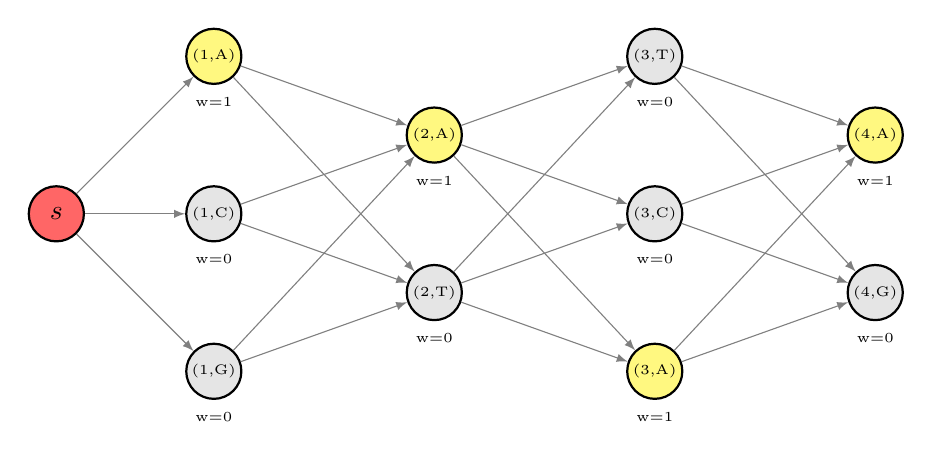
\begin{tikzpicture}[
            node distance=2.8cm and 1.0cm, % x distance and y distance
            node_style/.style={circle, draw, thick, minimum size=7mm, inner sep=0pt},
            weight_one/.style={node_style, fill=yellow!50},
            weight_zero/.style={node_style, fill=gray!20},
            source_node/.style={node_style, fill=red!60},
            edge_style/.style={->, >=latex, thin, gray},
            level_label/.style={font=\footnotesize, below=12mm of #1}
        ]

        % Nodes arranged by level (k) vertically aligned
        \node[source_node] (s) at (0, 0) {$s$};

        % Vertices for k=1 (X1 = {A, C, G})
        \node[weight_one] (v1A) at (2, 2) {\tiny (1,A)}; \node[below=1pt of v1A] {\tiny w=1};
        \node[weight_zero](v1C) at (2, 0) {\tiny (1,C)}; \node[below=1pt of v1C] {\tiny w=0};
        \node[weight_zero](v1G) at (2,-2) {\tiny (1,G)}; \node[below=1pt of v1G] {\tiny w=0};
        % \node[level_label=v1C] (l1) {$k=1$}; % Label for level 1

        % Vertices for k=2 (X2 = {A, T})
        \node[weight_one] (v2A) at (4.8, 1) {\tiny (2,A)}; \node[below=1pt of v2A] {\tiny w=1};
        \node[weight_zero](v2T) at (4.8,-1) {\tiny (2,T)}; \node[below=1pt of v2T] {\tiny w=0};
        % \node[level_label=v2A] (l2) {$k=2$}; % Label for level 2

        % Vertices for k=3 (X3 = {T, C, A})
        \node[weight_zero] (v3A) at (7.6, 2) {\tiny (3,T)}; \node[below=1pt of v3A] {\tiny w=0};
        \node[weight_zero](v3C) at (7.6, 0) {\tiny (3,C)}; \node[below=1pt of v3C] {\tiny w=0};
        \node[weight_one](v3T) at (7.6,-2) {\tiny (3,A)}; \node[below=1pt of v3T] {\tiny w=1};
        % \node[level_label=v3C] (l3) {$k=3$}; % Label for level 3

        % Vertices for k=4 (X4 = {A, G})
        \node[weight_one] (v4A) at (10.4, 1) {\tiny (4,A)}; \node[below=1pt of v4A] {\tiny w=1};
        \node[weight_zero](v4G) at (10.4,-1) {\tiny (4,G)}; \node[below=1pt of v4G] {\tiny w=0};
        % \node[level_label=v4A] (l4) {$k=4$}; % Label for level 4

        % Edges
        % s to Level 1
        \foreach \v in {v1A, v1C, v1G} { \draw[edge_style] (s) -- (\v); }

        % Level 1 to Level 2 (All-to-all)
        \foreach \u in {v1A, v1C, v1G} {
                \foreach \v in {v2A, v2T} {
                        \draw[edge_style] (\u) -- (\v);
                    }
            }

        % Level 2 to Level 3 (All-to-all)
        \foreach \u in {v2A, v2T} {
                \foreach \v in {v3A, v3C, v3T} {
                        \draw[edge_style] (\u) -- (\v);
                    }
            }

        % Level 3 to Level 4 (All-to-all)
        \foreach \u in {v3A, v3C, v3T} {
                \foreach \v in {v4A, v4G} {
                        \draw[edge_style] (\u) -- (\v);
                    }
            }

    \end{tikzpicture}
    \caption{The weighted DAG $G_A$ derived from the degenerate string in Figure \ref{fig:degenerate_example_tabular_v3} for character $c=\emph{A}$. Nodes visually labeled $(k,a)$ represent the vertices $v_{k,a}$. Nodes with $w_A(v_{k,a})=1$ are yellow; those with $w_A(v_{k,a})=0$ are gray. Edges represent the connections defined in $E_A$.}
    \label{fig:degenerate_dag_horizontal_v3}
\end{figure}

This graph-based perspective on degenerate strings serves as a concrete starting point for the core topic of this chapter: the development of succinct data structures for general node-weighted DAGs to support path-based queries. We address the challenge of representing an arbitrary DAG $G=(V, E, w)$, where each vertex $v \in V$ carries a non-negative integer weight $w(v)$, in a compressed format that efficiently supports queries related to cumulative path weights. Such weighted DAGs model various phenomena beyond degenerate strings. For example, in bioinformatics, pangenome graphs\footnote{Pangenome graphs may contain cycles. These cycles can be addressed by either removing them or by utilizing path information provided by modern pangenome graph formats.} can be interpreted through this lens: if each node corresponds to a DNA sequence (a string over $\{A, C, G, T\}$), the weight $w(v)$ could represent the count of a specific nucleotide (e.g., \emph{A}) within that sequence; similarly for \emph{C}, \emph{G}, and \emph{T}.

Our primary focus is on generalizing the \Rank{} query to this graph setting; the \textsf{select} query, while definable, will not be treated further in this work. For a given vertex $N$, the \textsf{rank} query aims to describe the set of possible cumulative weights achievable on paths originating from a designated source vertex $s$ and terminating at $N$.

The combinatorial complexity of paths in a DAG - potentially exponential in the number of vertices - makes naive approaches based on explicit path enumeration or storage infeasible for large graphs. This motivated us to development of a \emph{succinct} data structure. Our approach involves partitioning the vertices based on how their path weight information is represented: some vertices (\emph{explicit}) will store this information directly, while others (\emph{implicit}) will rely on indirect derivation through references facilitated by a carefully defined \emph{successor} relationship, as detailed in Section \ref{sec:succinct_dag_representation}.

% --- SLIDE 9: Connecting Degenerate Strings to DAGs ---
\begin{frame}{From Degenerate Strings to Weighted DAGs}
    \framesubtitle{A New Perspective}

    Recall our degenerate string $X$:
    \begin{figure}[h!]
        \centering
        % Usa la figura della stringa degenere che hai già definito
        \begin{tabular}{c@{\hskip 0.5em}c@{\hskip 0.5em}c@{\hskip 0.5em}c@{\hskip 0.5em}c}
            $X = $                                                                           & $\Bigg\{\,\begin{matrix}\texttt{A}\\\texttt{C}\\\texttt{G}\end{matrix}\,\Bigg\}$ &
            $\Bigg\{\,\begin{matrix}\texttt{A}\\\texttt{T}\end{matrix}\,\Bigg\}$             &
            $\Bigg\{\,\begin{matrix}\texttt{T}\\\texttt{C}\\\texttt{A}\end{matrix}\,\Bigg\}$ &
            $\Bigg\{\,\begin{matrix}\texttt{A}\\\texttt{G}\end{matrix}\,\Bigg\}$                                                                                                                        \\
                                                                                             & $X_1$                                                                            & $X_2$ & $X_3$ & $X_4$
        \end{tabular}
    \end{figure}

    \uncover<2->{
        \begin{block}{Key Idea}
            We can model queries on $X$ by constructing a specific node-weighted Directed Acyclic Graph (DAG) $G_c$ for a target character $c$.
        \end{block}
    }

    \uncover<3->{
        \begin{itemize}
            \item<3-> \textbf{Vertices $V_c$}: Source $s$ + one node $v_{k,a}$ for each character $a \in X_k$ at each position $k$.
            \item<4-> \textbf{Weights $w_c$}: $w_c(s)=0$. $w_c(v_{k,a}) = 1$ if $a = c$, else $0$. (Highlights occurrences of $c$).
            \item<5-> \textbf{Edges $E_c$}: Connect $s$ to $k=1$. Connect all $v_{k,a}$ to all $v_{k+1,b}$. (Represents sequence adjacency).
        \end{itemize}
    }

\end{frame}

% --- SLIDE 10: Path Weight Aggregation: The O-Set Definition ---
\begin{frame}{Path Weight Aggregation: The $\mathcal{O}$-Set}
    \framesubtitle{Capturing All Path Weights}
    Given a path $P=(v_0=s, \dots, v_k=v)$ we define $W(P) = \sum_{j=1}^{k} w(v_j)$
    \begin{alertblock}{Goal}
        Characterize the set of \alert{all possible distinct} cumulative path weights arriving at each node.
    \end{alertblock}
    % \vspace{1em}
    \pause
    \begin{block}{$\mathcal{O}$-Set Definition (Recursive)}
        \begin{itemize}
            \item \textbf{Base Case (Source):} $\mathcal{O}_s = \{0\}$
            \item \textbf{Recursive Step ($v \neq s$):}
                  \[ \mathcal{O}_v = \bigcup_{u \in Pred(v)} \{ y + w(v) \mid y \in \mathcal{O}_u \} = \{ W(P) \mid P \in Path(s, v) \}  \]
                  Keep only \alert{distinct} values. Store as a sorted sequence.
        \end{itemize}
    \end{block}
    % The set $\mathcal{O}_v$ contains \emph{exactly} the weights $W(P)$ for all paths $P$ from source $s$ to $v$.
    % \[ \mathcal{O}_v = \{ W(P) \mid P \in Path(s, v) \} \]

\end{frame}

% --- SLIDE 11: O-Set Construction Example ---
\begin{frame}{$\mathcal{O}$-Set Construction Example}
    \framesubtitle{Visualizing the Recursive Definition}
    \vspace{-0.5em}
    \begin{figure}[hbtp]
        % \centering
        % Replace TikZ with sequential images
        \only<1>{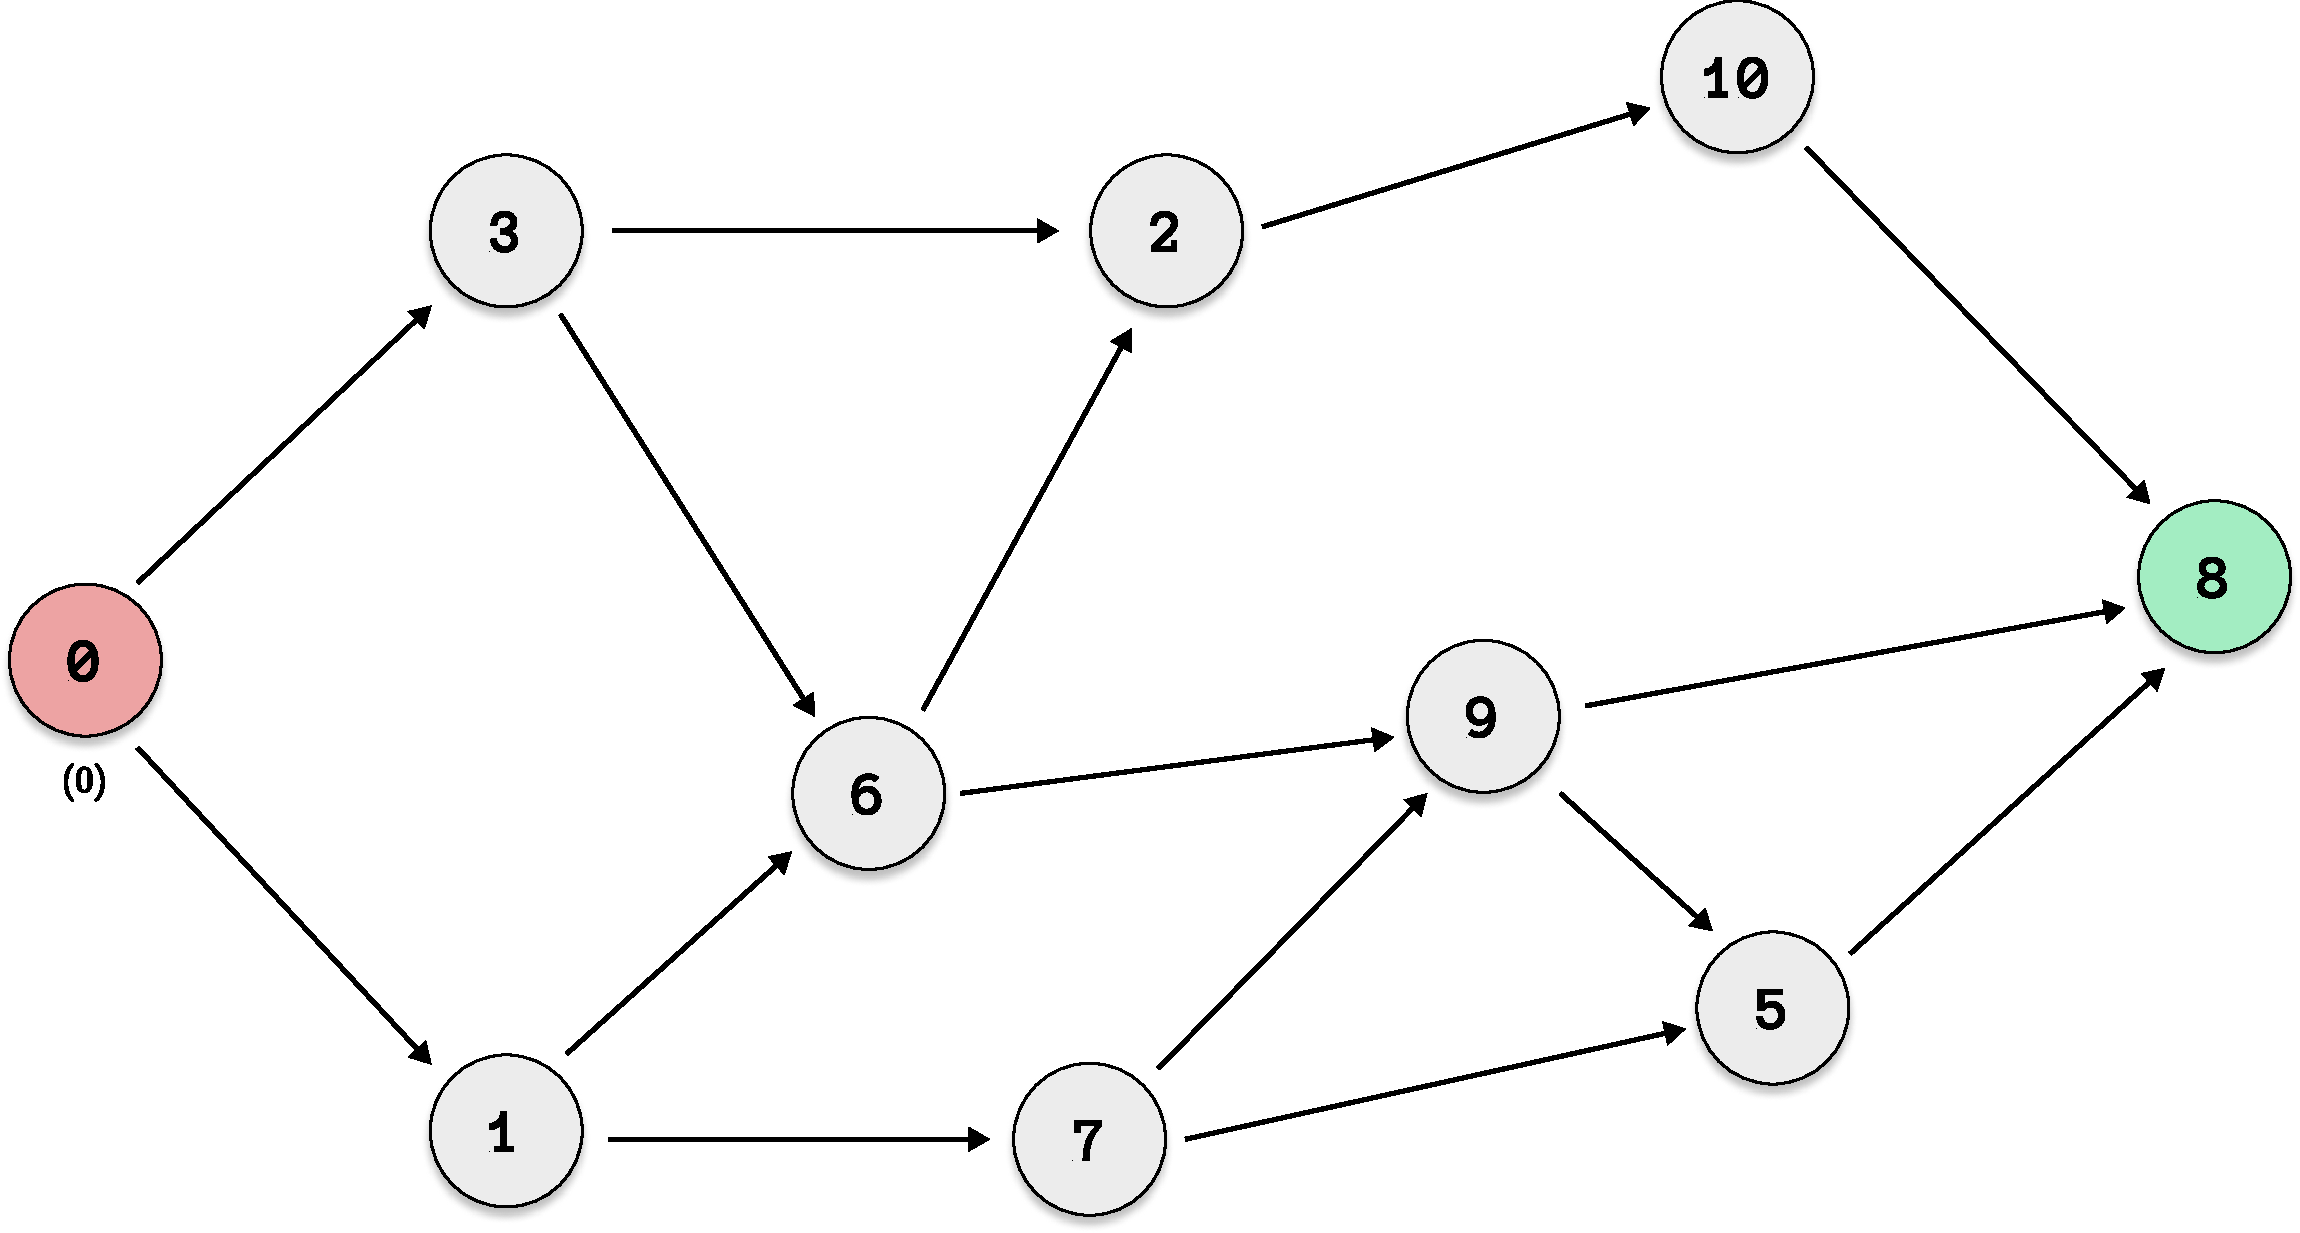
\includegraphics[width=0.85\textwidth]{assets/dag_explicit1.pdf}}
        % \only<2>{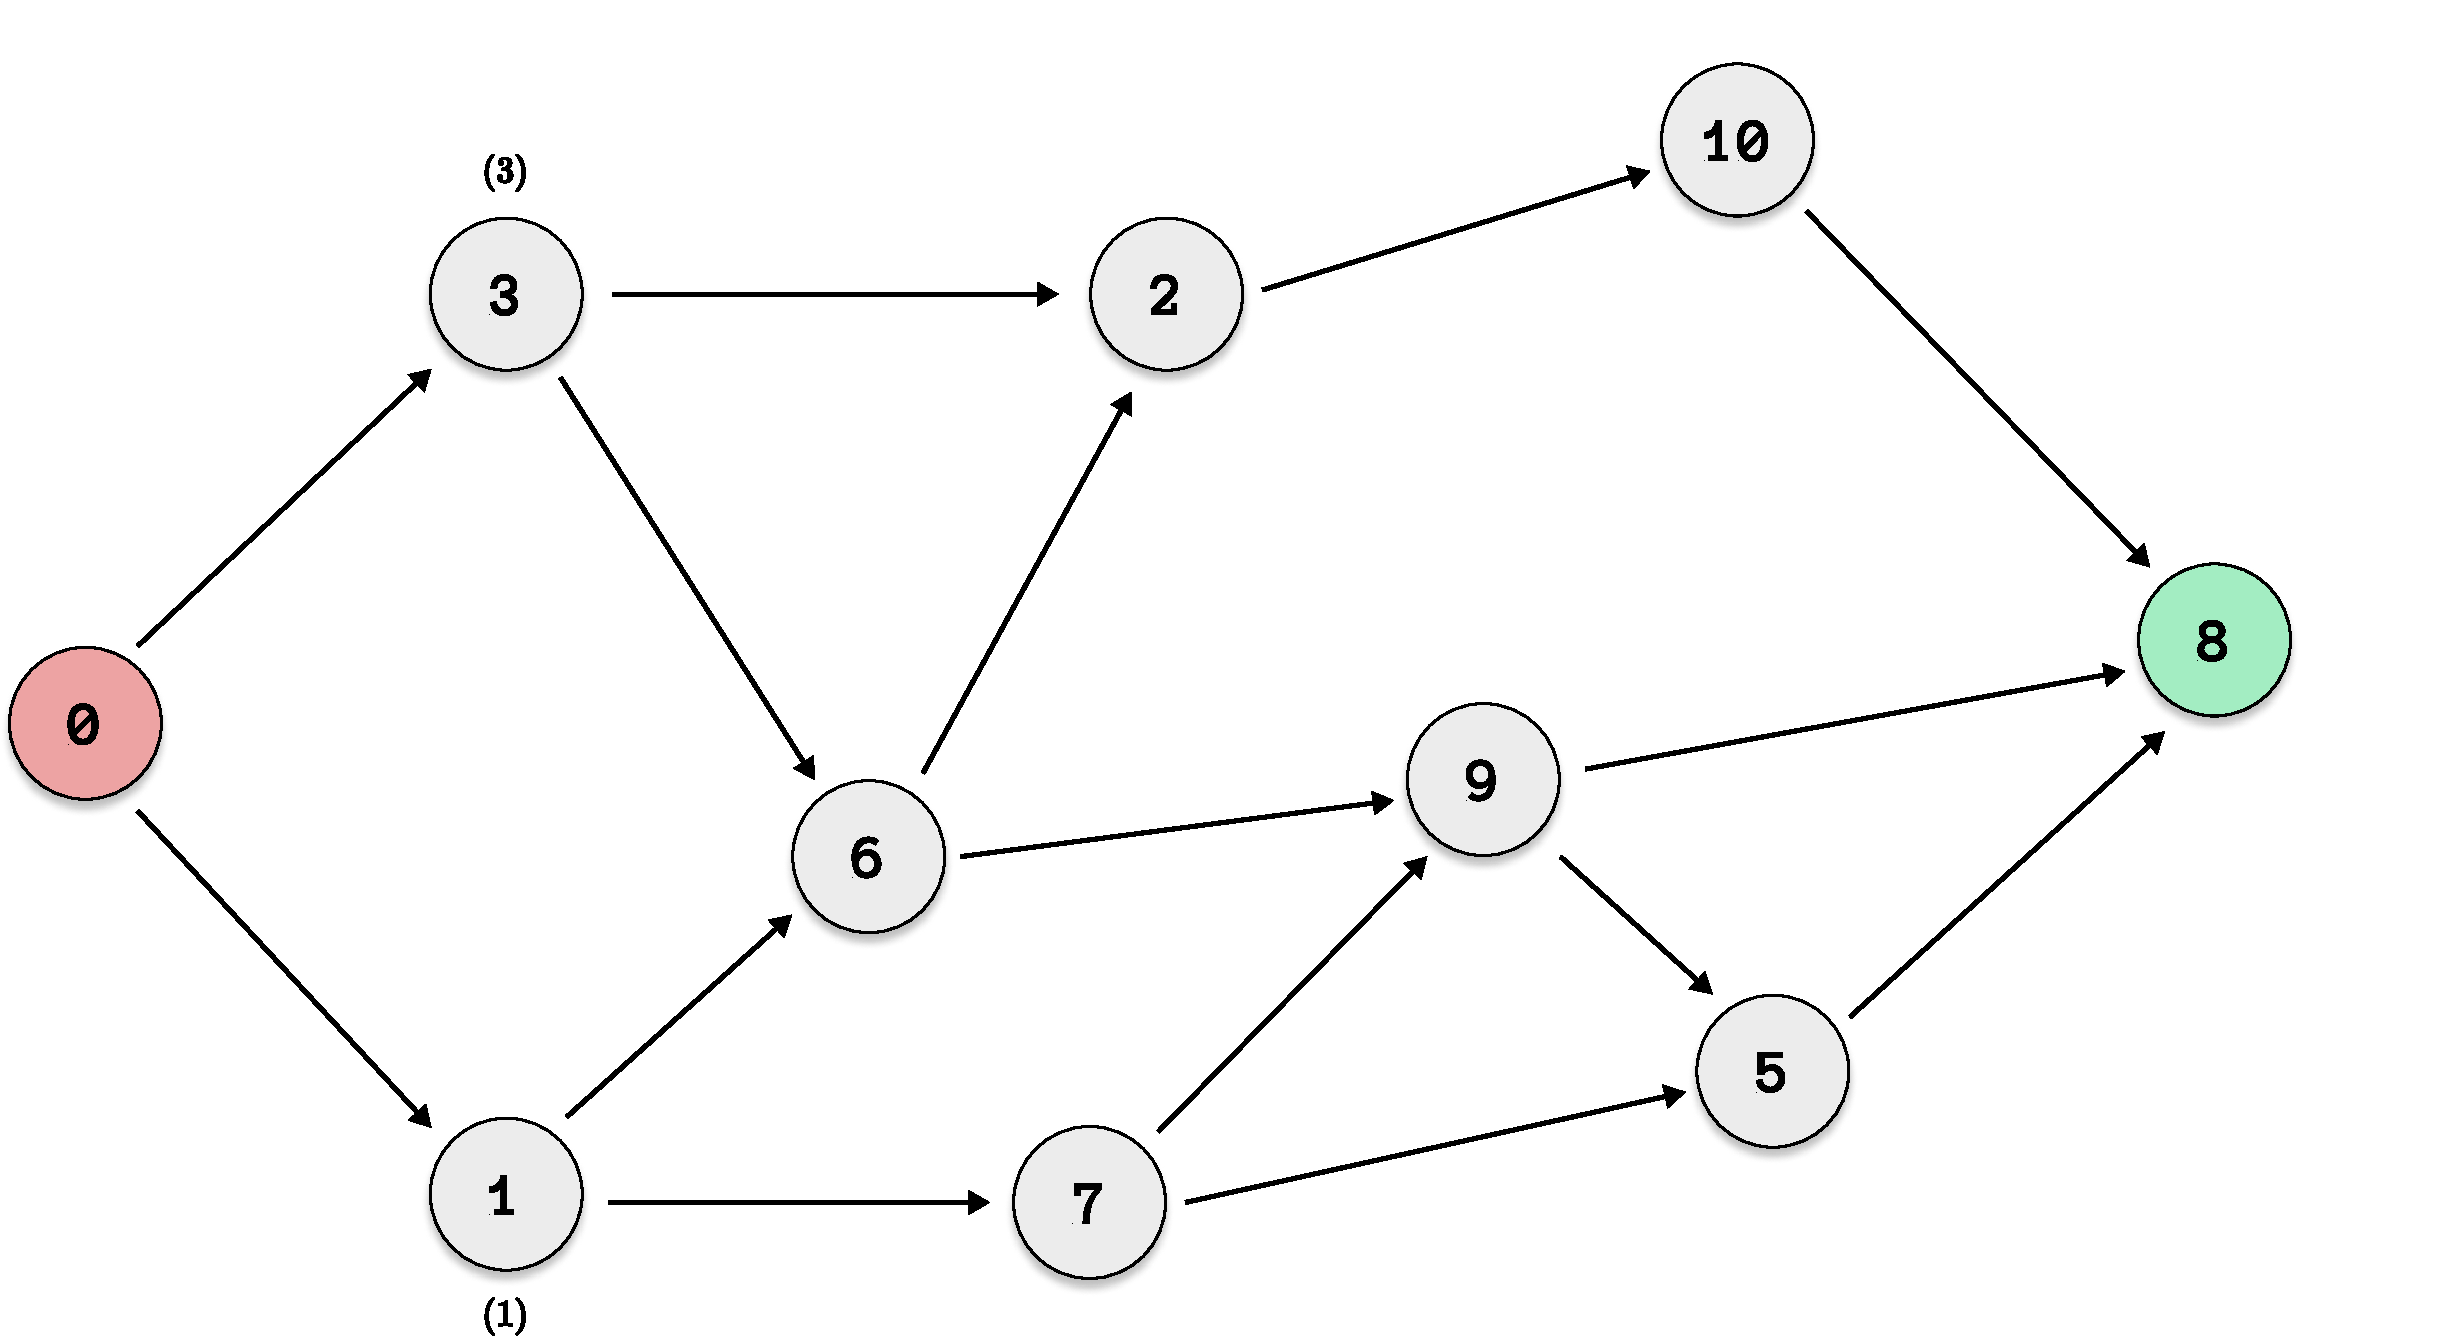
\includegraphics[width=0.85\textwidth]{assets/dag_explicit2.pdf}}
        \only<2>{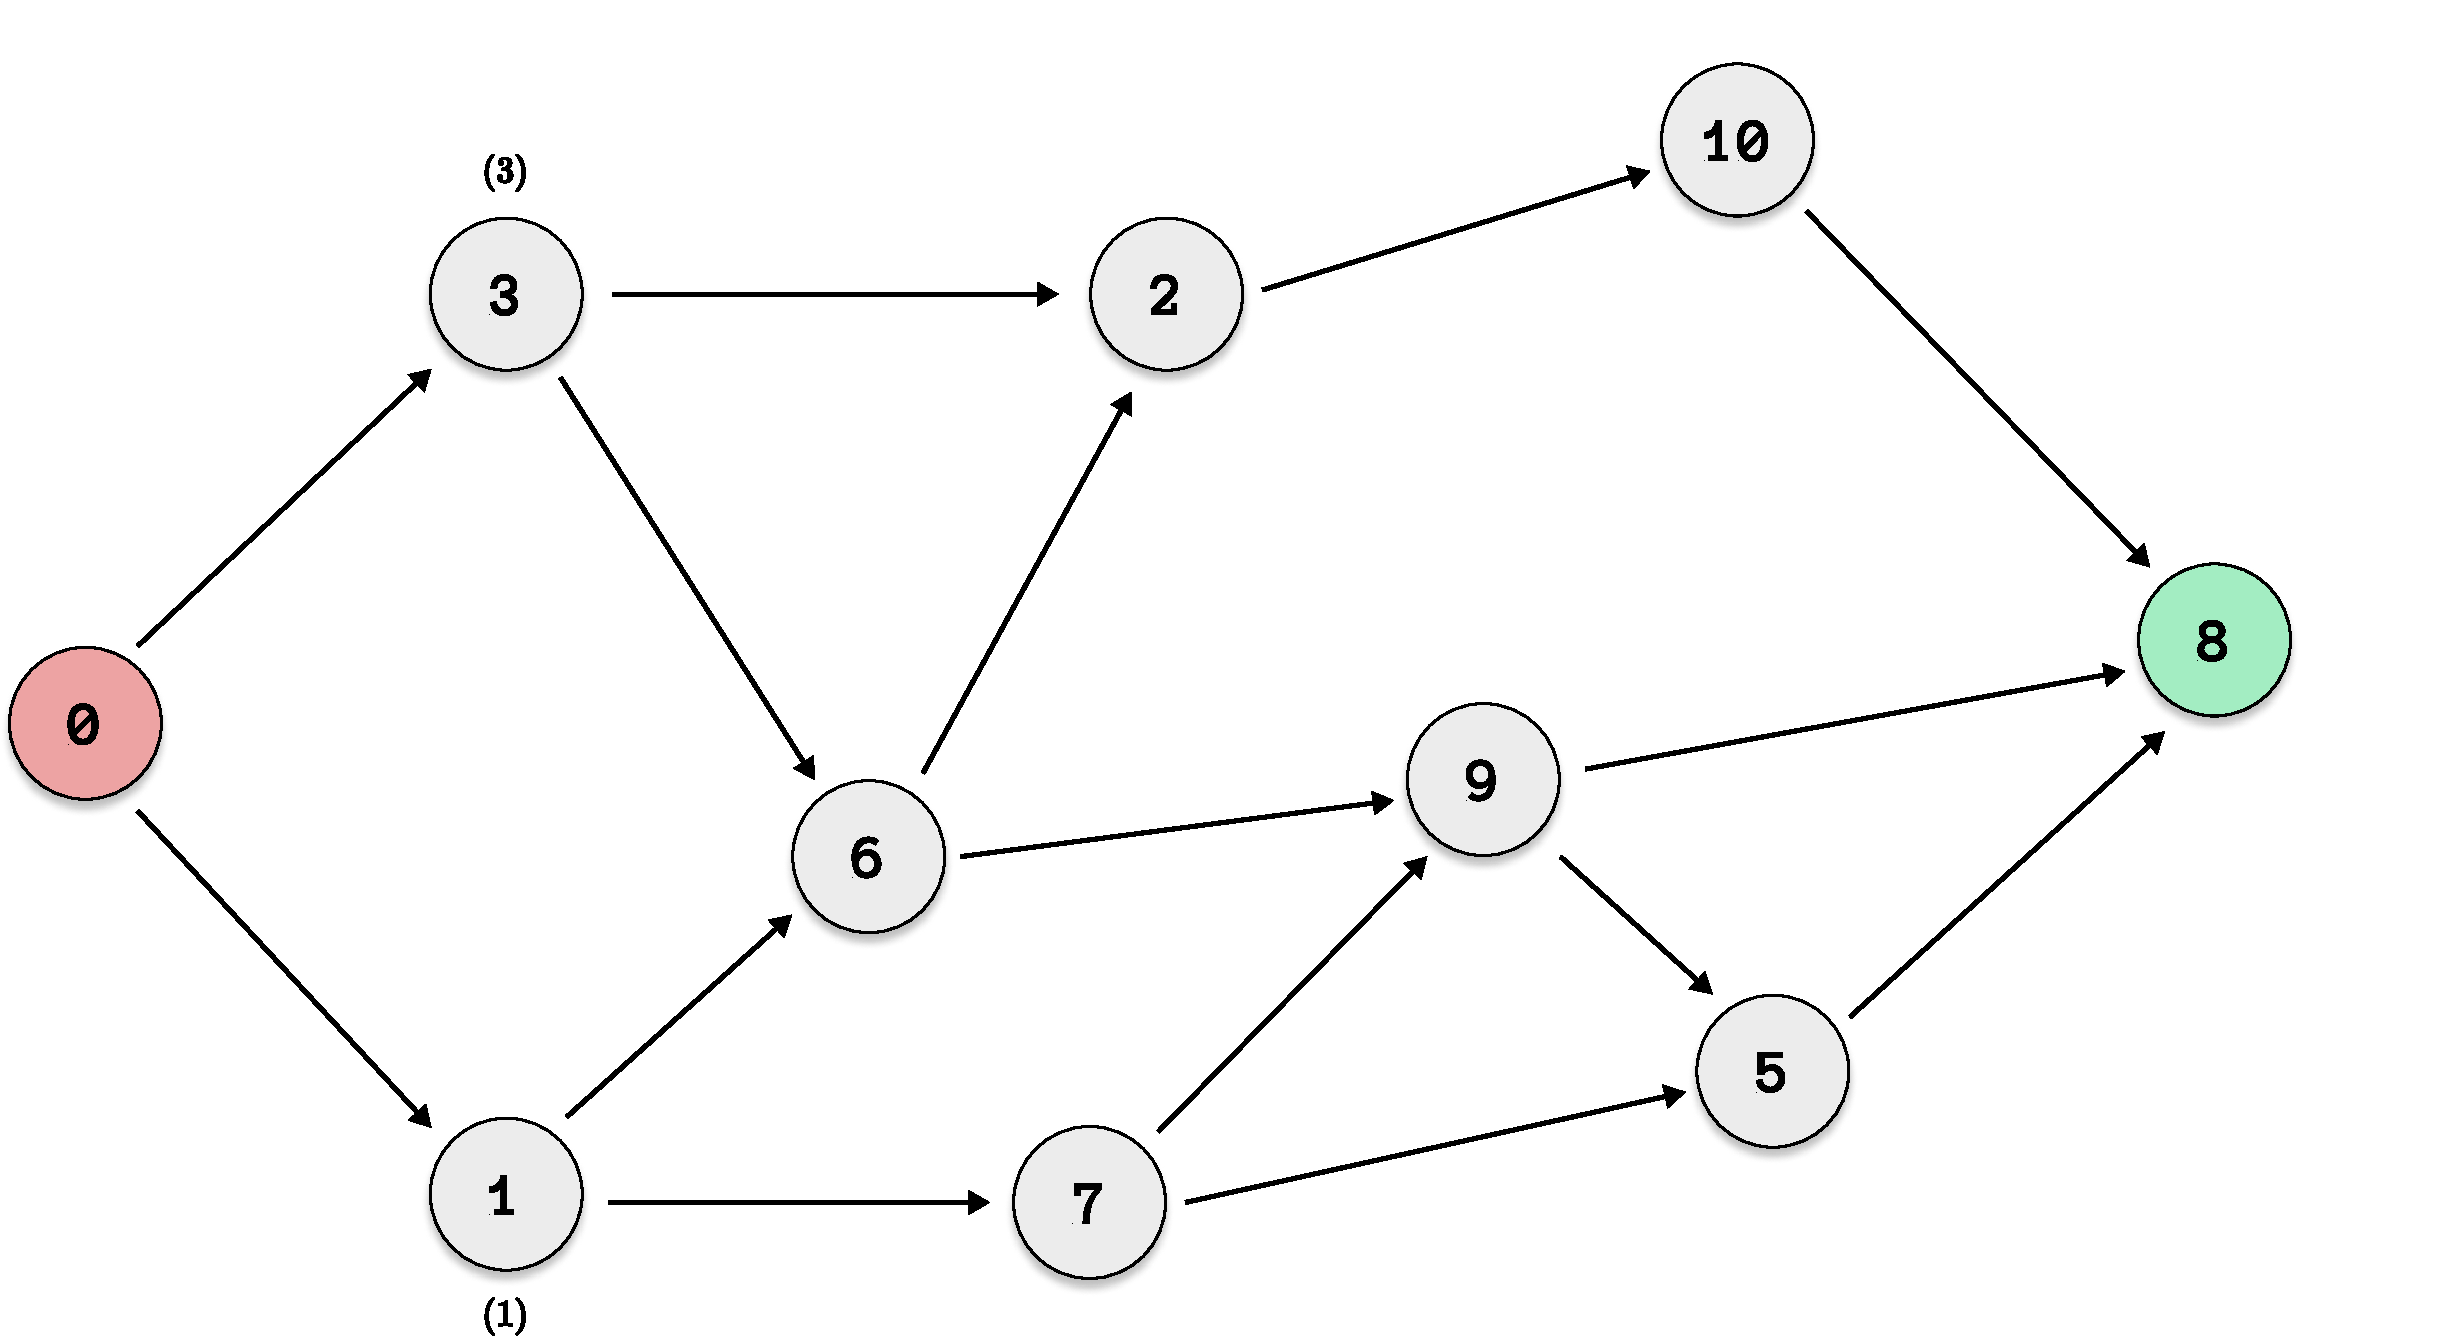
\includegraphics[width=0.85\textwidth]{assets/dag_explicit3.pdf}}
        \only<3>{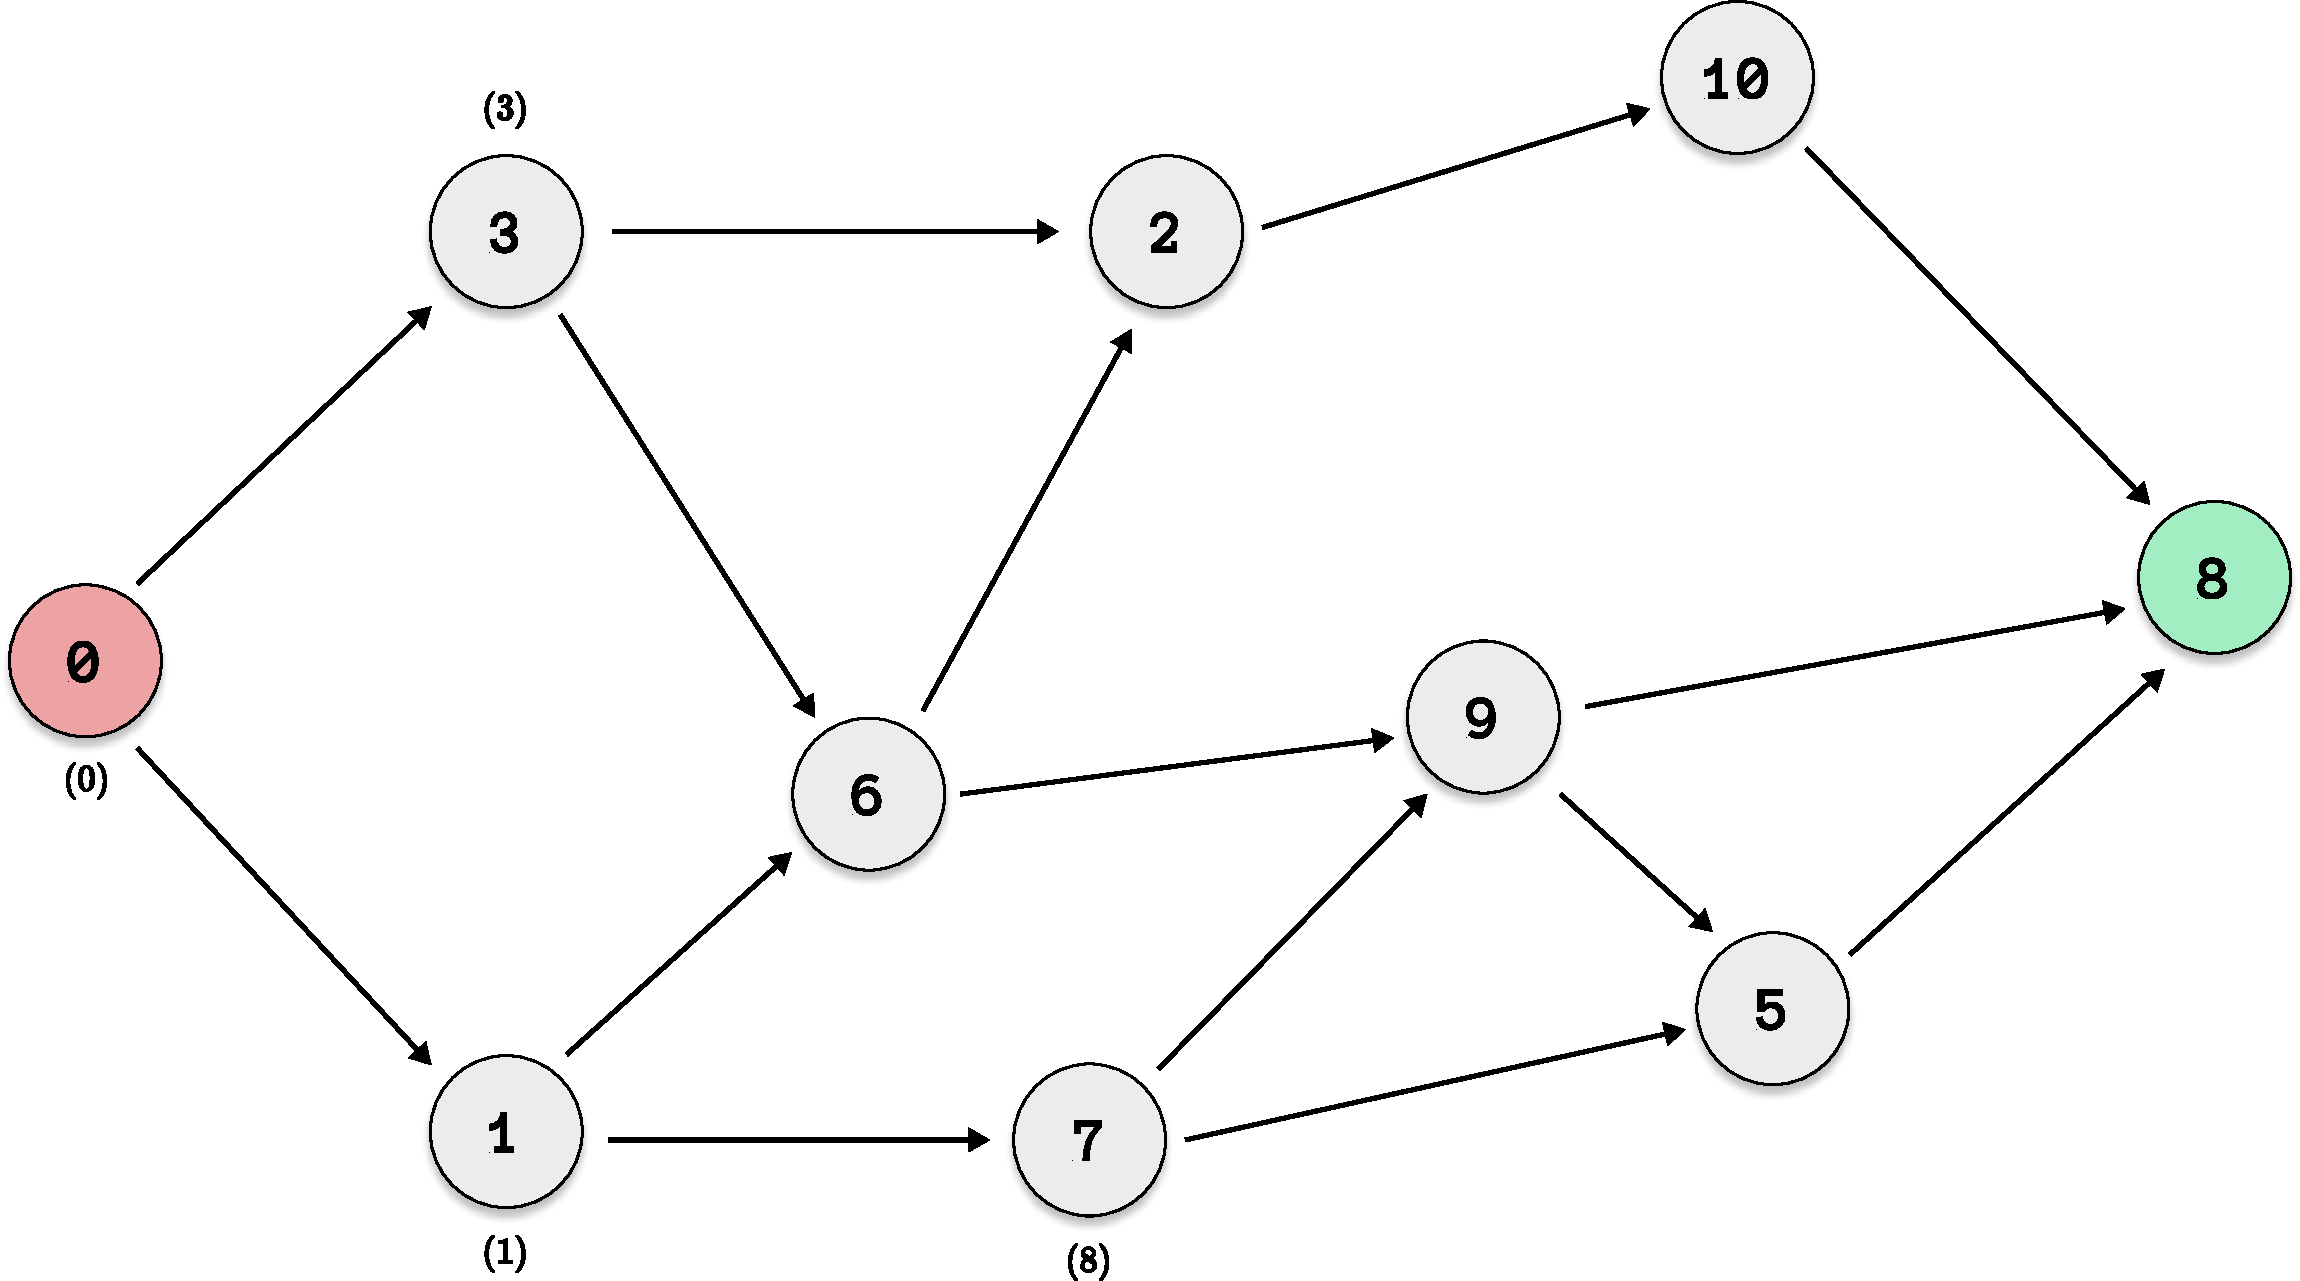
\includegraphics[width=0.85\textwidth]{assets/dag_explicit4.pdf}}
        \only<4>{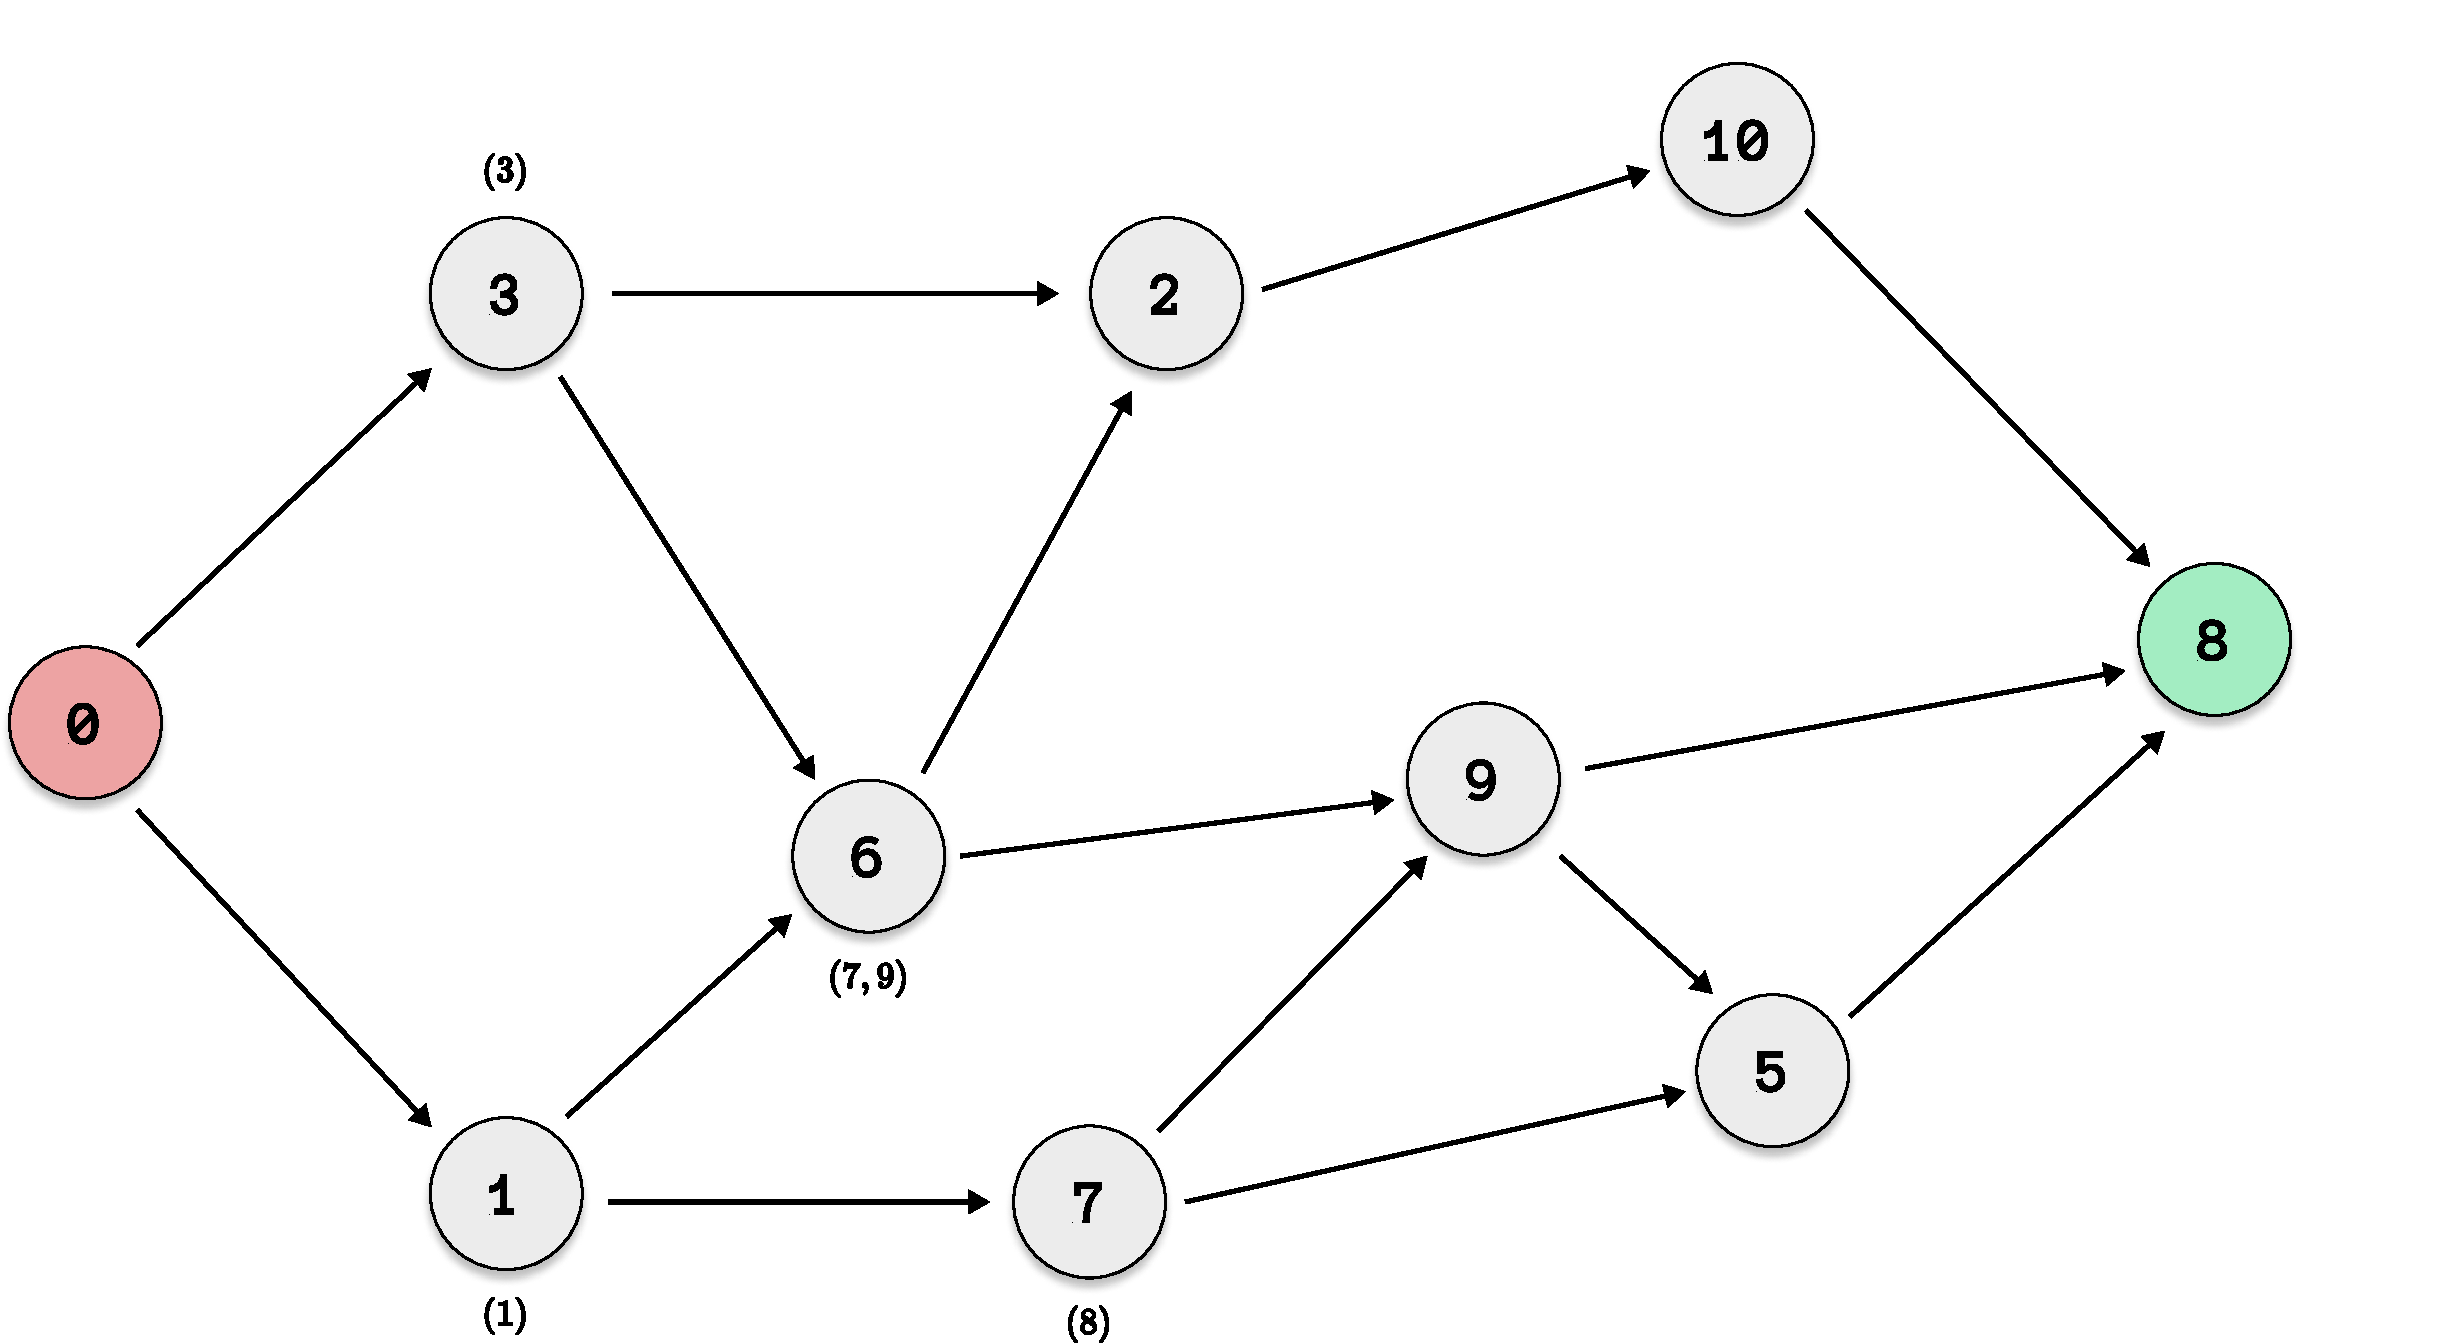
\includegraphics[width=0.85\textwidth]{assets/dag_explicit5.pdf}}
        \only<5>{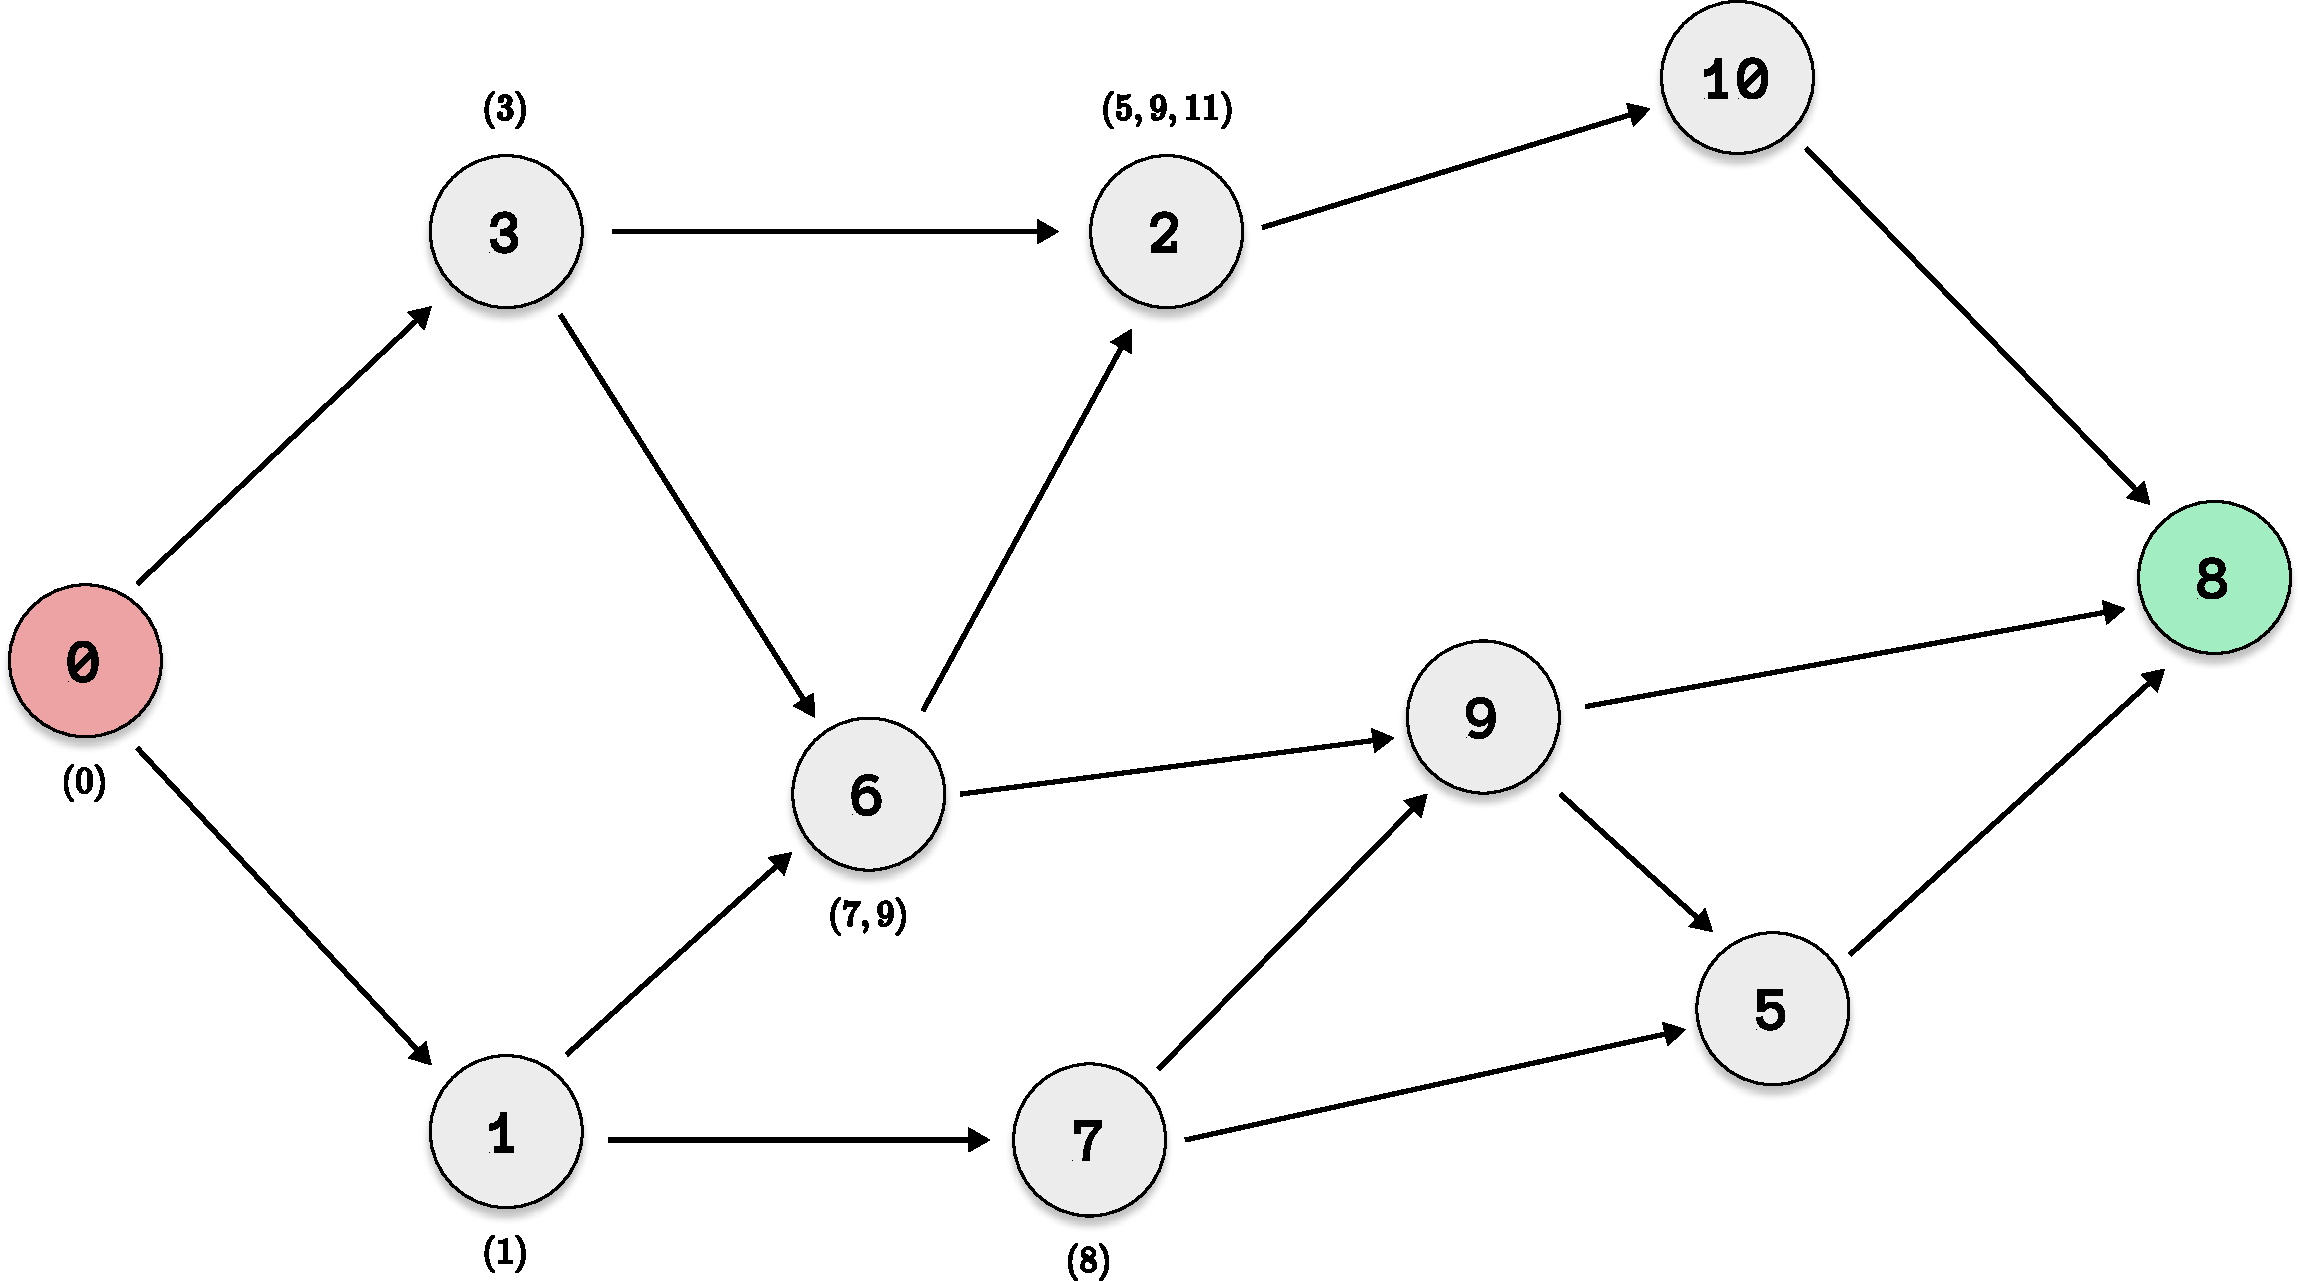
\includegraphics[width=0.85\textwidth]{assets/dag_explicit6.pdf}}
        \only<6>{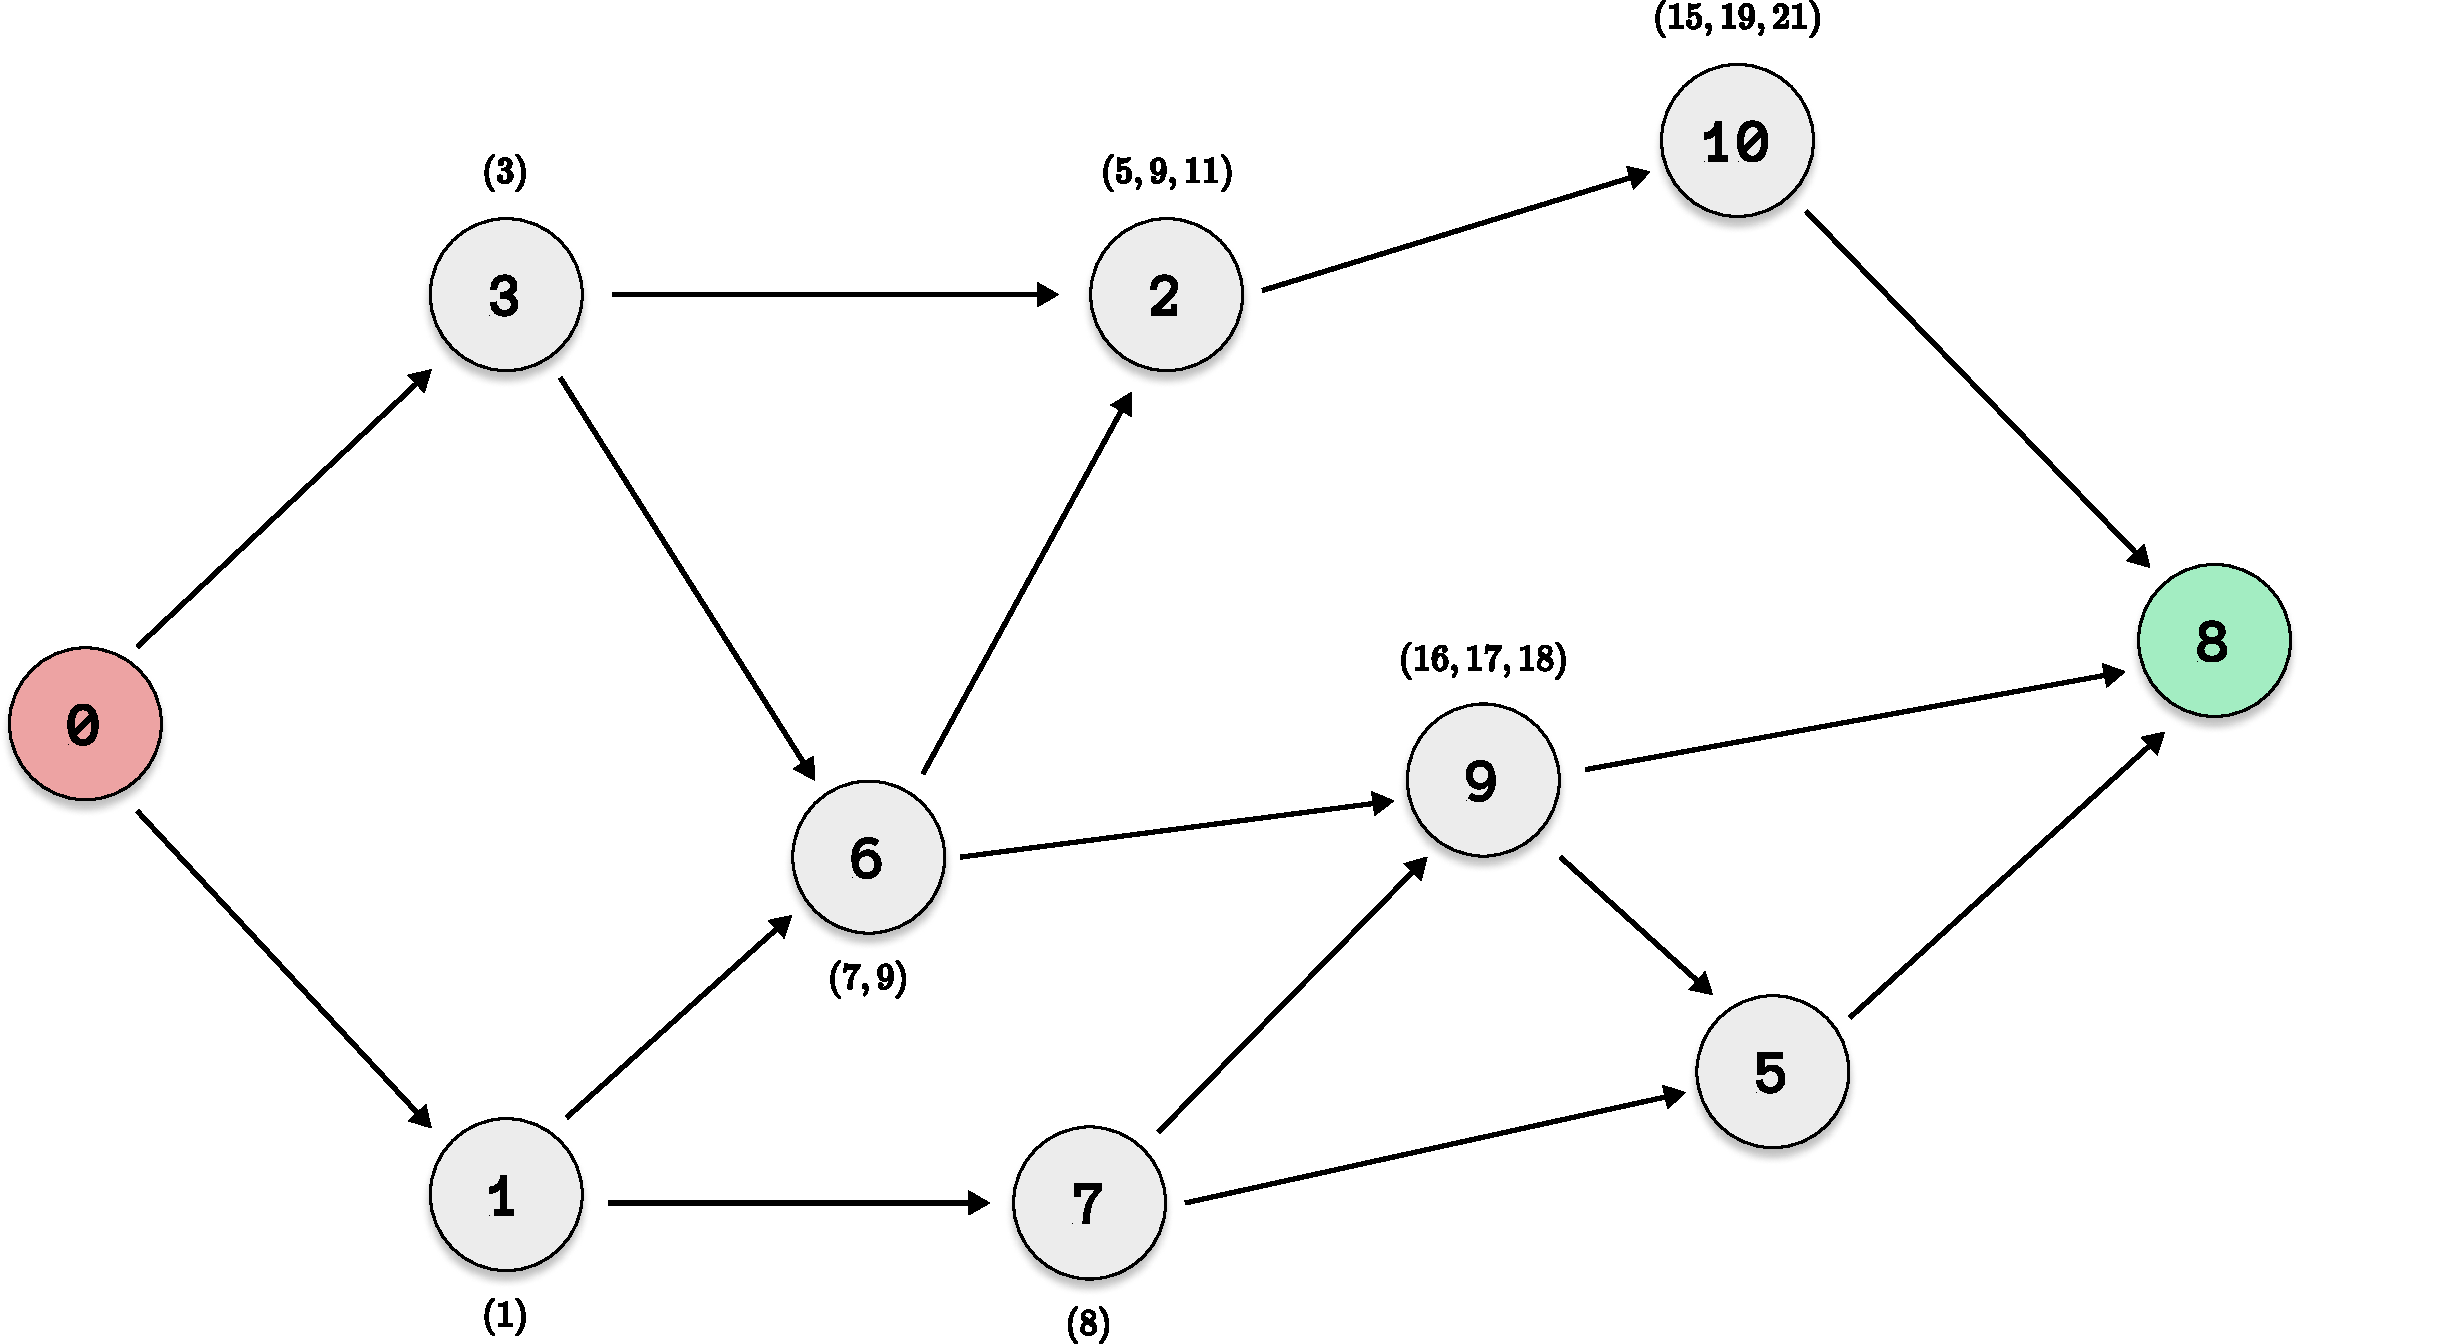
\includegraphics[width=0.85\textwidth]{assets/dag_explicit7.pdf}}
        \only<7>{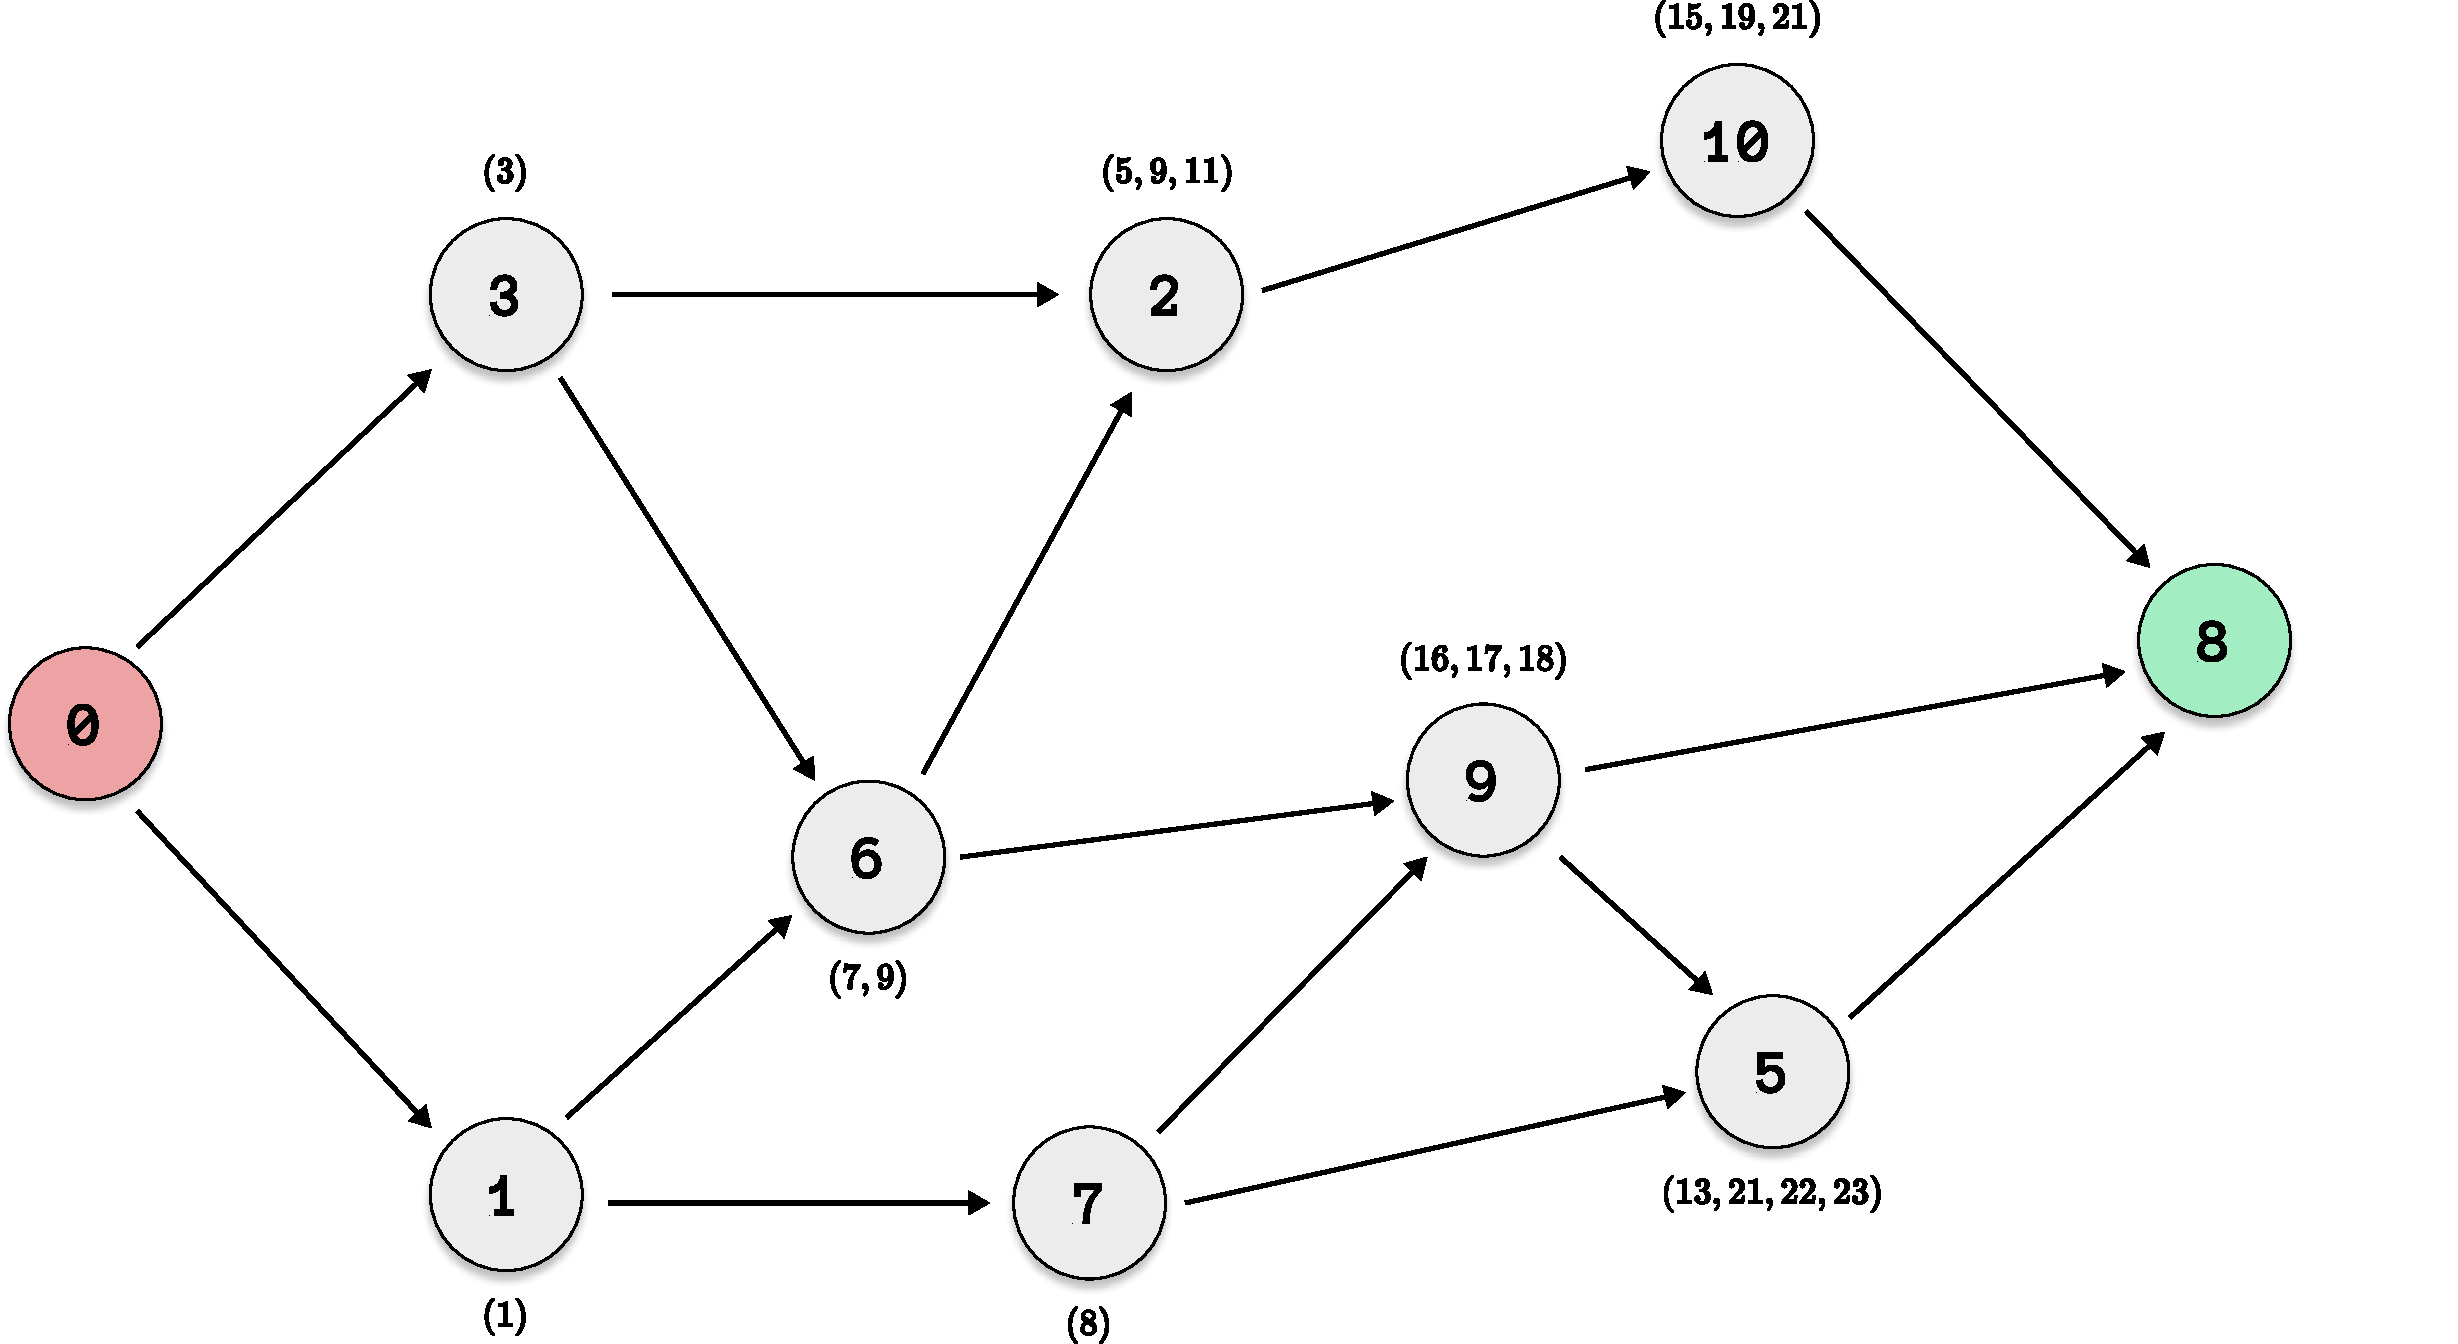
\includegraphics[width=0.85\textwidth]{assets/dag_explicit8.pdf}}
        \only<8>{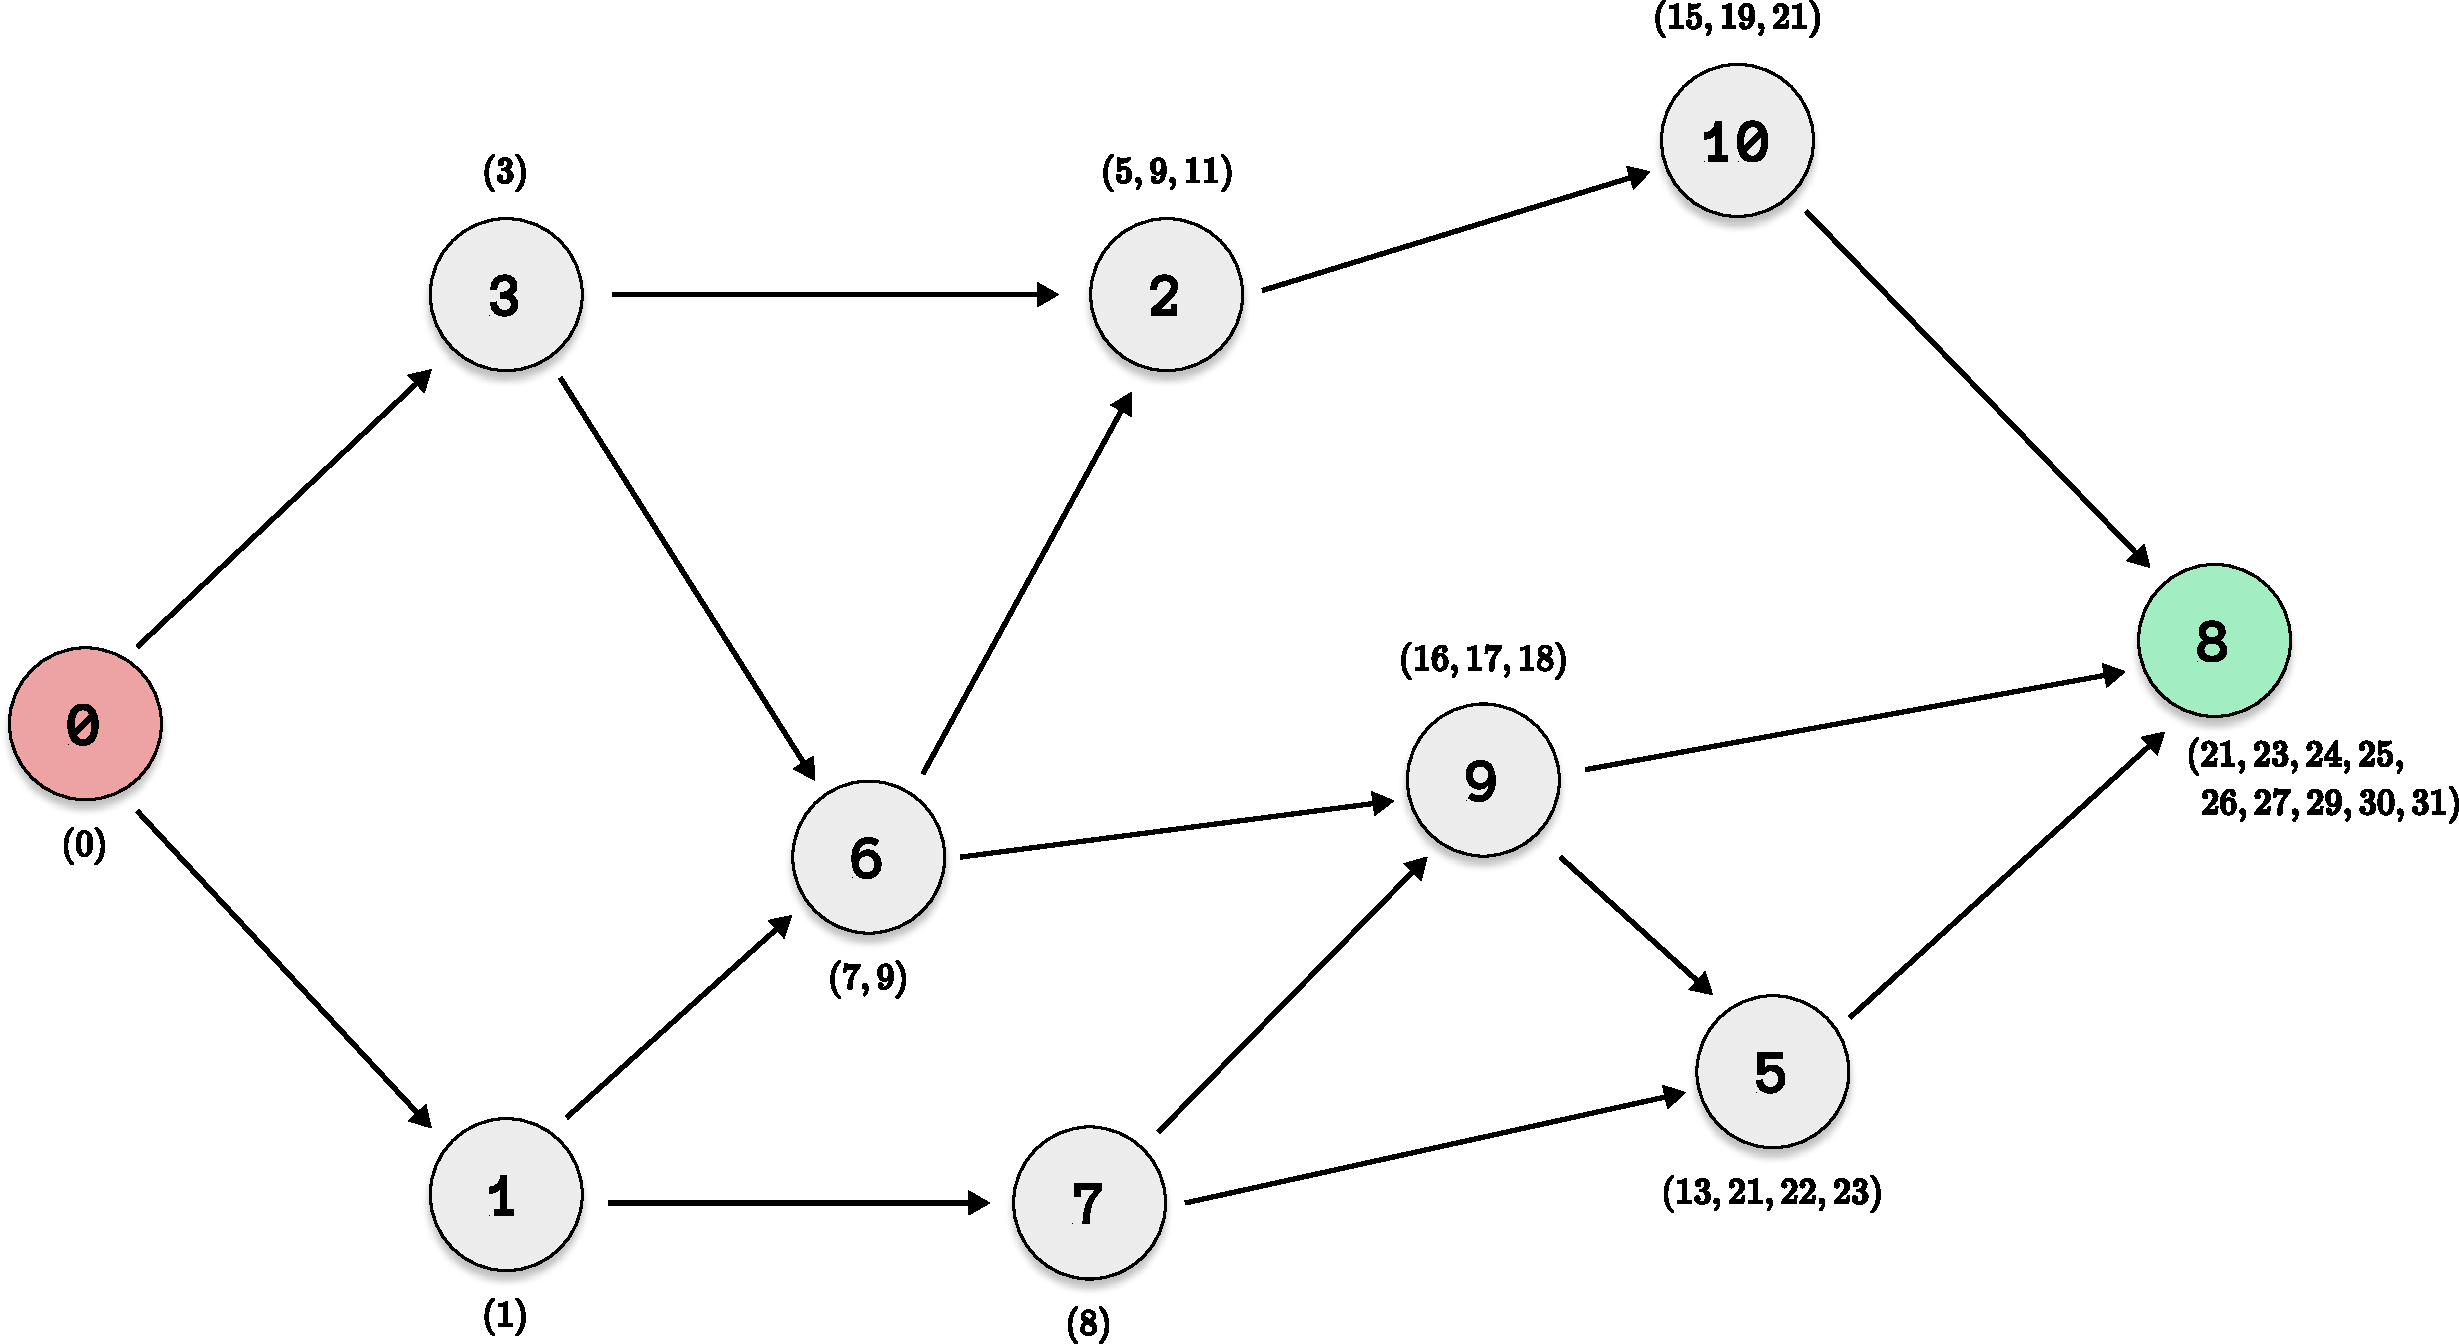
\includegraphics[width=0.85\textwidth]{assets/dag_explicit_final.pdf}}
    \end{figure}
    % \begin{figure}[h!]
    %     \centering
    %     % \resizebox{0.9\textwidth}{!}{% Reduced size slightly to make space for labels
    %     %     \begin{tikzpicture}[
    %     %         node distance=1.5cm and 1cm,
    %     %         base_node/.style={circle, draw=black, thick, minimum size=8mm, inner sep=0pt, font=\sffamily},
    %     %         root_node/.style={base_node, fill=red!60, text=black},
    %     %         % Definizione stile per label O-set
    %     %         data_label/.style={font=\tiny\ttfamily, text=blue!80!black, anchor=north},
    %     %         edge_style/.style={->, >={Stealth[length=2mm]}, thick, draw=black}
    %     %         ]

    %     %         % Nodes (pesi dentro)
    %     %         \node[root_node] (0) at (0, 2) {0};
    %     %         \node[base_node] (1) at (1.5, 0) {1};
    %     %         \node[base_node] (3) at (1.5, 4) {3};
    %     %         \node[base_node] (6) at (3.5, 1.5) {6};
    %     %         \node[base_node] (7) at (4.5, 0) {7};
    %     %         \node[base_node] (2) at (5.5, 4) {2};
    %     %         \node[base_node] (9) at (6.5, 2) {9};
    %     %         \node[base_node] (5) at (9, 0.5) {5};
    %     %         \node[base_node] (10) at (8.5, 5) {10};
    %     %         \node[base_node] (8) at (11, 3) {8};

    %     %         % Edges
    %     %         \draw [edge_style] (0) -- (1); \draw [edge_style] (0) -- (3);
    %     %         \draw [edge_style] (1) -- (6); \draw [edge_style] (1) -- (7);
    %     %         \draw [edge_style] (3) -- (2); \draw [edge_style] (3) -- (6);
    %     %         \draw [edge_style] (6) -- (2); \draw [edge_style] (6) -- (9);
    %     %         \draw [edge_style] (7) -- (5); \draw [edge_style] (7) -- (9);
    %     %         \draw [edge_style] (2) -- (10);
    %     %         \draw [edge_style] (9) -- (5); \draw [edge_style] (9) -- (8);
    %     %         \draw [edge_style] (10) -- (8); \draw [edge_style] (5) -- (8);

    %     %         % O-Set Labels appearing step-by-step
    %     %         \node<1->[data_label, red] at (0.south) {\{0\}};
    %     %         \node<2->[data_label] at (1.south) {\{1\}};
    %     %         \node<2->[data_label] at (3.south) {\{3\}};
    %     %         \node<3->[data_label] at (7.south) {\{8\}};
    %     %         \node<4->[data_label] at (6.south) {\{7, 9\}};
    %     %         \node<5->[data_label] at ([xshift=0.3cm]2.south) {\{5, 9, 11\}};
    %     %         \node<6->[data_label] at ([yshift=-0.1cm, xshift=0.2cm]9.south) {\{16, 17, 18\}};
    %     %         \node<7->[data_label] at (10.south) {\{15, 19, 21\}};
    %     %         \node<8->[data_label] at (5.south) {\{13, 21, 22, 23\}};
    %     %         \node<9->[data_label, align=center] at ([yshift=-0.2cm, xshift=0.4cm]8.south) {\{21, 23, 24, 25, \\ 26, 27, 29, 30, 31\}};

    %     %     \end{tikzpicture}
    %     % } % End resizebox
    % \end{figure}
\end{frame}

% --- SLIDE 12: The Rank Query - Concept ---
\begin{frame}{The Rank Query on Weighted DAGs}
    \framesubtitle{What Values are "Active" at Node N?}
    % \begin{block}{Motivation}
    %     The $\mathcal{O}$-Set ($\mathcal{O}_N$) tells us the \alert{final} path weights ending at node $N$.
    %     But we want to know which cumulative weight values are relevant \alert{during} the "processing" step associated with node $N$ itself.
    % \end{block}
    \begin{block}{Rank Query on a Node $N$: $\mathrm{rank}_G(N)$}
        \begin{enumerate}
            \item Returns a representation of a set of integers derived from the $\mathcal{O}$-set $\mathcal{O}_N$.
                  \[ S_N = \bigcup_{x \in \mathcal{O}_N} \{ z \in \mathbb{N}_0 \mid \max(0, x - w(N) + 1) \le z \le x \}. \]
                  \vspace{-1em}
                  \pause
            \item These intervals are then maximally merged. The query $\mathrm{rank}_G(N)$ returns a \alert{minimal collection of disjoint closed integer intervals}
                  \[ \mathcal{R}_N = \{[l_1, r_1], [l_2, r_2], \dots, [l_p, r_p]\} \]
                  such that their union exactly covers $S_N$.
                  % \item Return the result as a \alert{minimal set of disjoint intervals} $\mathcal{R}_N$.
        \end{enumerate}
    \end{block}
    $\mathcal{R}_N$ captures the range of possible cumulative sums during the \emph{activity} at node $N$

\end{frame}

% --- SLIDE 13: The Challenge: Storing Path Information ---
\begin{frame}{The Challenge: Storing Path Information}
    \framesubtitle{$\mathcal{O}$-Sets Can Be Huge!}

    % Problema e Domanda rimangono uguali
    \begin{itemize}
        \item \textbf{Problem}: The size $|\mathcal{O}_v|$ can grow very large!
        \item \textbf{Question:} Can we represent the necessary information more compactly?
    \end{itemize}


    \begin{alertblock}<2->{Core Idea: Partitioning + Indirection}
        Partition vertices $V$ into two types:
    \end{alertblock}
    \vspace{-1em}
    \begin{columns}[T] % T allinea al top
        \begin{column}{0.48\textwidth}
            \begin{block}<2->{1. Explicit Vertices ($V_E$)}
                \centering
                Store $\mathcal{O}_v$ directly. \\
                (\textit{Simple, but potentially large})
            \end{block}
            % \uncover<3->{\textbf{}
        \end{column}

        \begin{column}{0.48\textwidth}
            \begin{block}<2->{2. Implicit Vertices ($V_I$)}
                \centering
                Do \emph{not} store $\mathcal{O}_v$ explicitly \\
                (\textit{Reconstruct on-the-fly.})
            \end{block}
            \vspace{0.5em}
        \end{column}
    \end{columns}
    \uncover<3->{\textbf{Reconstruction for $v \in V_I$ using}:
        \begin{itemize}
            \item Designated Successor $\sigma(v)$
            \item Offset Sequence $\mathcal{J}_v$ (at $v$)
        \end{itemize}
    }
\end{frame}

% --- SLIDE 14: Successor Choice and Offset Sequence ---
\begin{frame}{Implicit Reconstruction: Successor \& Offset}
    \framesubtitle{How $V_I$ Nodes Refer to Others}

    \begin{block}{1. Designated Successor $\sigma(v)$ (for $v \in V_I$)}
        Which successor should $v$ point to?
        \textbf{Heuristic}: Choose $u = \sigma(v)$ that minimizes $|\mathcal{O}_u|$.
        \[ \sigma(v) \in \underset{u \in Succ(v)}{\operatorname{argmin}} \{ |\mathcal{O}_u| \}. \]
    \end{block}
    \begin{block}{2. Offset Sequence $\mathcal{J}_v$ (for $v \in V_I$)}
        How to get $\mathcal{O}_v$ from $\mathcal{O}_{\sigma(v)}$? Let $u=\sigma(v)$.
        \begin{itemize}
            % \item Property: We know $|\mathcal{O}_v| \le |\mathcal{O}_u|$.
            \item \textbf{Relationship}: Each element $x_k \in \mathcal{O}_v$ comes from some $y_{j_k} \in \mathcal{O}_u$ via $x_k = y_{j_k} - w(u)$.
            \item \textbf{Offset Sequence $\mathcal{J}_v$}: Stores the index $j_k$ corresponding to each $x_k$.
                  \[ \mathcal{J}_v = (j_0, j_1, \dots, j_{m-1}), \quad \text{where } m = |\mathcal{O}_v| \]
        \end{itemize}
    \end{block}

\end{frame}

% --- SLIDE 15: Example: Computing O_9[1] (Static Structure First) ---
\begin{frame}{Example: Computing $\mathcal{O}_9[1]$}
    \framesubtitle{Following the Successor Path: $9 \to 5 \to 8$}
    \begin{figure}[hbtp]
        \centering
        % Replace TikZ with sequential images
        \only<1>{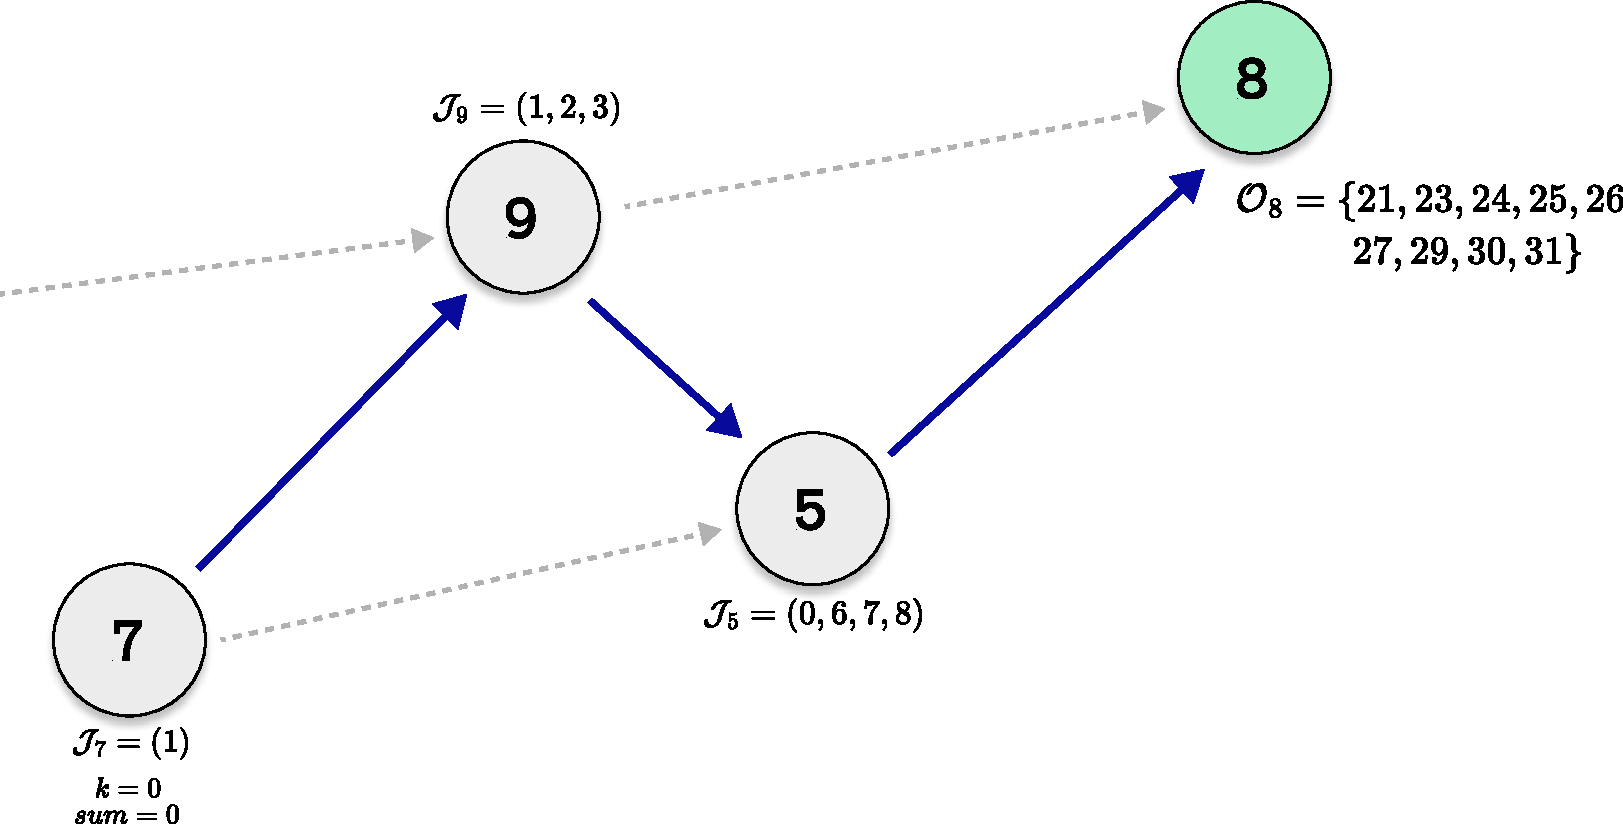
\includegraphics[width=0.9\textwidth]{assets/dag_query1.pdf}}
        \only<2>{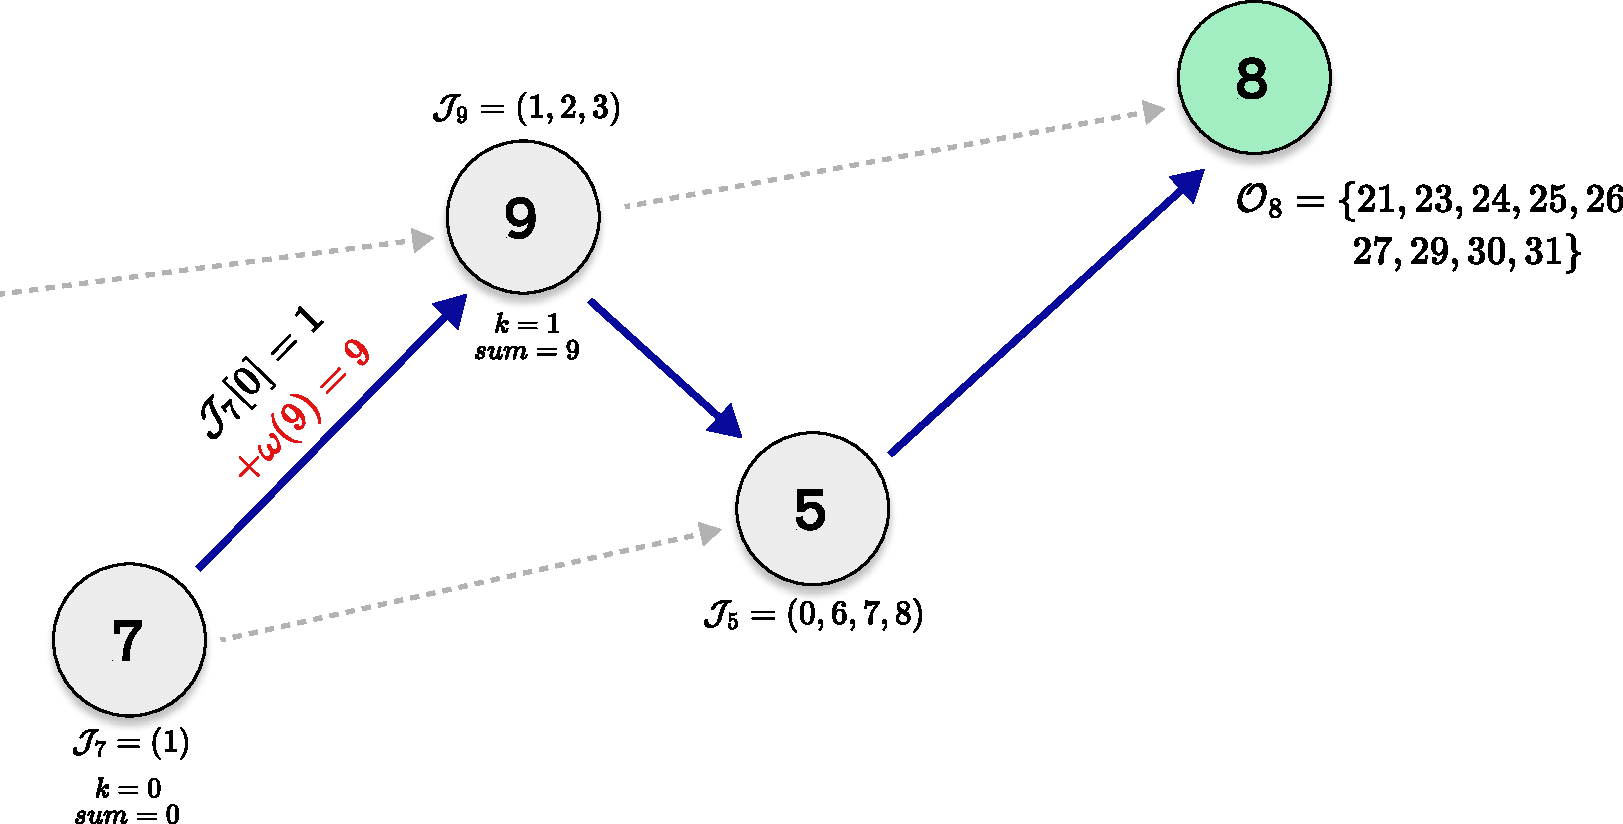
\includegraphics[width=0.9\textwidth]{assets/dag_query2.pdf}}
        \only<3>{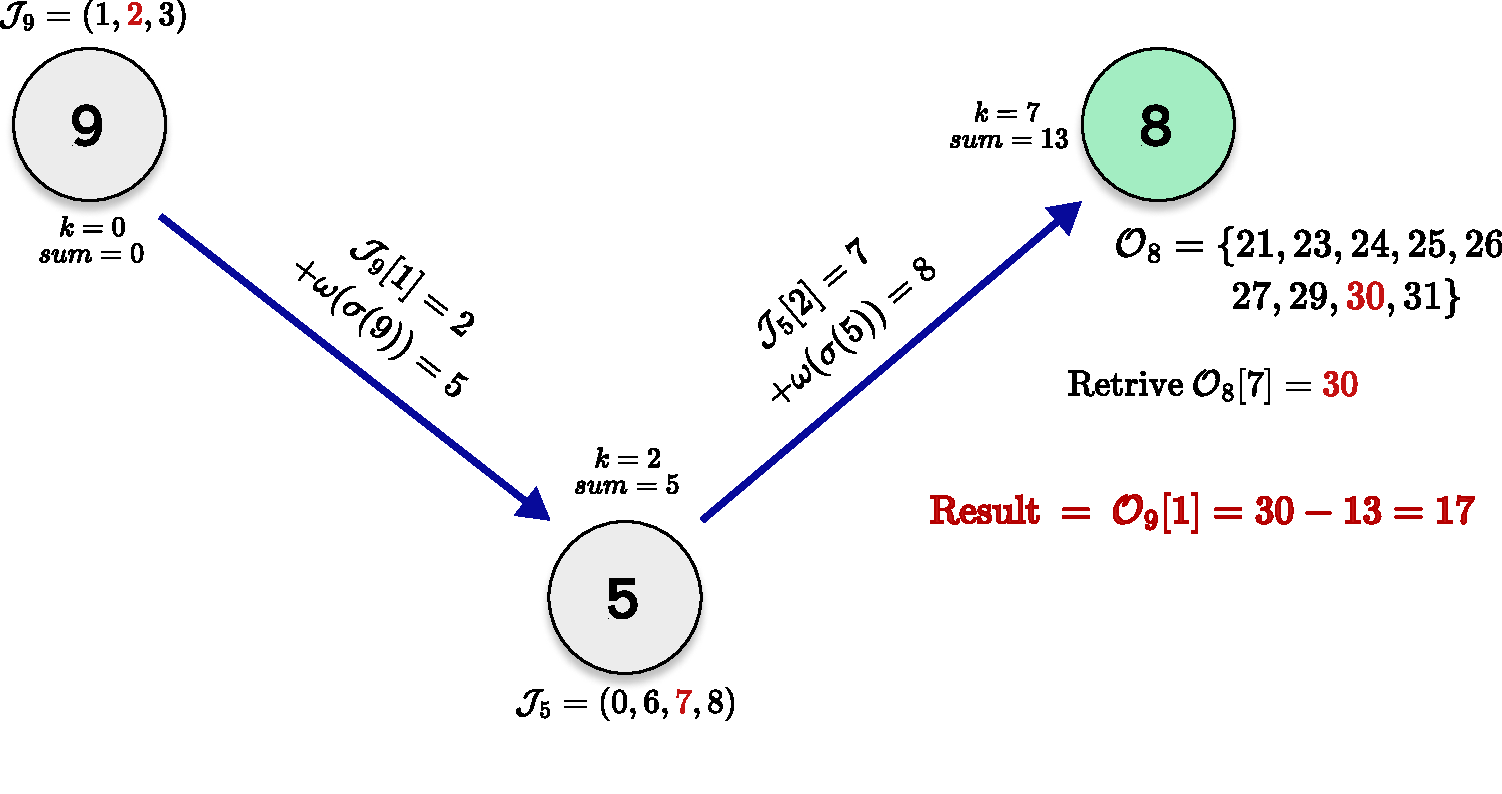
\includegraphics[width=0.9\textwidth]{assets/dag_query3.pdf}}
        % \only<4>{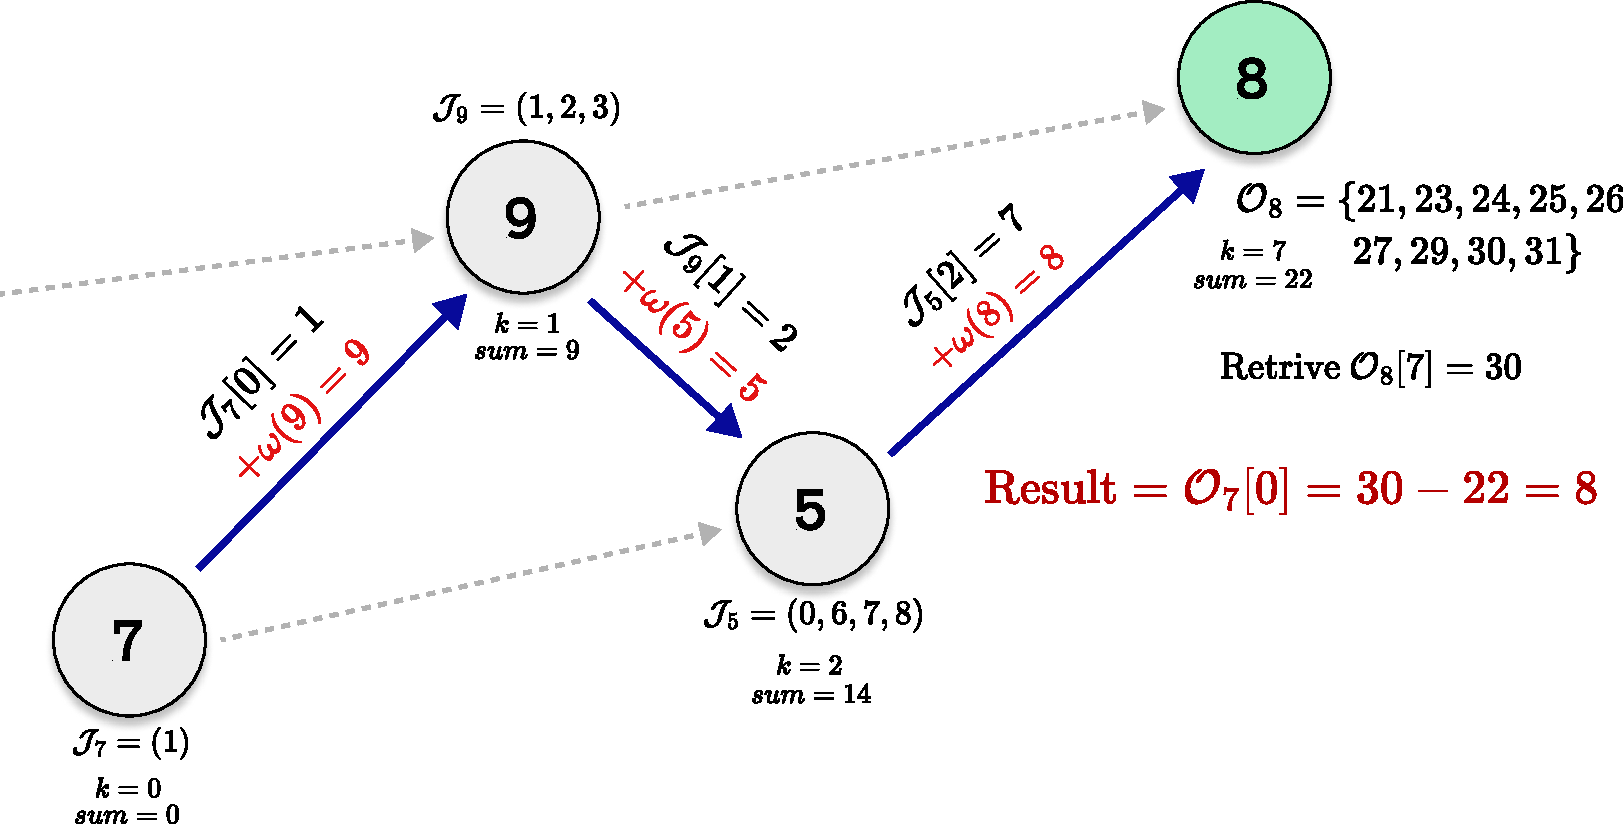
\includegraphics[width=0.9\textwidth]{assets/dag_query4.pdf}}
    \end{figure}
\end{frame}

% --- SLIDE 16: Example: Computing O_7[0] (Dynamic Structure) ---
\begin{frame}{Succinct Data Structure: Components}
    \framesubtitle{Arrays Indexed by Vertex ID}
    % divide in two columns
    \begin{columns}[T]
        \column{0.5\textwidth}
        \uncover<1->{\begin{center}
                \textbf{Each node stores 3 components}
            \end{center}
            \begin{center}
                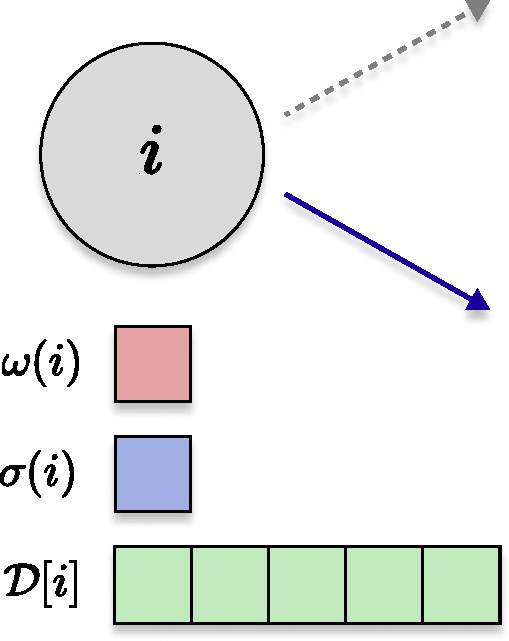
\includegraphics[width=0.55\textwidth]{assets/AoS.pdf}
            \end{center}}

        \column{0.5\textwidth}
        \uncover<2->{\begin{center}
                \textbf{Succinct DAG as a Struct of Arrays}
            \end{center}
            \begin{center}
                \vspace{0.5em}
                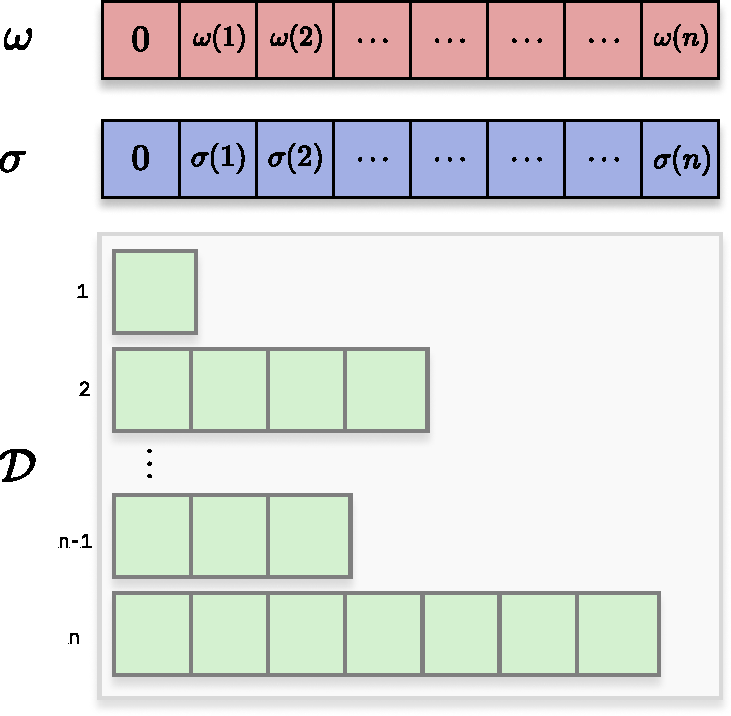
\includegraphics[width=0.8\textwidth]{assets/SoA.pdf}
            \end{center}}
    \end{columns}
\end{frame}

% --- SLIDE 17: Compression Strategies - Overview ---
\begin{frame}{Compression Strategies}
    \framesubtitle{Reducing Memory Footprint}
    \begin{center}
        \begin{tabular}{l l}
            \toprule
            \textbf{Component}              & \textbf{Description}                             \\
            \midrule
            % Le prime due righe appaiono insieme al passo 1
            \uncover<1->{%
            $\mathcal{W}$ (Node weights)    & Array of positive integers.                      \\
            } % Appare dalla slide 1 in poi
            \uncover<1->{%
            $\Sigma$ (Successor IDs)        & Array of positive integers.                      \\
            } % Appare dalla slide 1 in poi
            % L'ultima riga e la linea inferiore appaiono al passo 3
            \uncover<3->{%
            $\mathcal{D}$ (Associated Data) & Array of arrays of increasing positive integers. \\
                \bottomrule
            } % Appare dalla slide 3 in poi
        \end{tabular}
    \end{center}
    \vspace{-1.5em}
    % Il blocco alert appare al passo 2, insieme ai primi due item
    \begin{alertblock}{Compression Options}<2-> % Appare dalla slide 2 in poi
        \begin{itemize}
            % I primi due item appaiono al passo 2
            \item<2-> Variable-Length Integer Coding $\longrightarrow$ we published a Rust library\footnote[1]{\url{https://crates.io/crates/compressed-intvec}} for this! % Appare dalla slide 2 in poi
            \item<2-> Wavelet Trees \emph{(for nodes with small weight range)} % Appare dalla slide 2 in poi
                % Gli ultimi due item appaiono al passo 4
            \item<4-> Elias-Fano Encoding \emph{(for monotonic sequences)} % Appare dalla slide 4 in poi
            \item<4-> Run-Length Encoding (RLE) \emph{(for clustered monotonic sequences)} % Appare dalla slide 4 in poi
        \end{itemize}
    \end{alertblock}
\end{frame}

% --- SLIDE 18: Baseline: Graph Entropy H0(G) ---
\begin{frame}{Space Efficiency: Baseline Comparison}
    \framesubtitle{How Much Information is in the Graph?}
    To evaluate our structure's space, \alert{we need a baseline}.
    \begin{block}<1->{$0^{th}$-Order Graph Entropy $H_0(G)$}
        A theoretical lower bound for storing the \emph{entire} weighted DAG ($V, E, w$) losslessly.
        \[ H_0(G) = \underbrace{H_W(G)}_{\text{Cost for Weights}} + \underbrace{H_E(G)}_{\text{Cost for Topology (Edges)}} \]
    \end{block}
    \begin{itemize}
        \item<2-> $H_W(G) \approx \sum_{v \in V} \log(w(v)+1)$ bits (\emph{Minimal binary encoding for weights}).
        \item<3-> $H_E(G) \approx \log \binom{n(n-1)}{m}$ bits (\emph{Cost to choose $m=|E|$ edges out of all possible $n(n-1)$}).
    \end{itemize}
    \vspace{0.5em}
    \uncover<4->{\textbf{Any method saving the \emph{full} graph structure needs at least $H_0(G)$ bits!}}

\end{frame}

% --- SLIDE 19: Space Comparison - Key Numbers ---
\begin{frame}{Space Comparison: Succinct Structure vs. Baselines}
    \framesubtitle{Bitcoin DAG Example ($n \approx 22k, m \approx 50k$)}
    \begin{columns}[c] % Keep [t] for top alignment
        \begin{column}{0.5\textwidth} % Adjusted width potentially
            \centering
            \begin{tabular}{l r}
                \toprule
                \textbf{Method}                       & \textbf{Estimated Bits}          \\
                \midrule
                \textbf{Theoretical Lower Bound}      & \uncover<1->{\textbf{1,525,730}} \\
                \quad Weights $H_W(G)$                & \uncover<1->{60,824}             \\
                \quad Topology $H_E(G)$               & \uncover<1->{1,464,906}          \\
                \midrule
                \textit{Precomputed Rank Queries:}    &                                  \\
                \quad Explicit Binary Storage         & \uncover<2->{4,854,533}          \\
                \quad Elias-Fano Compressed           & \uncover<2->{2,211,849}          \\
                \midrule
                \textbf{Our Succinct DAG}             & \uncover<3->{\textbf{602,808}}   \\
                \quad Weights $\mathcal{W}$           & \uncover<3->{60,824}             \\
                \quad Successors $\Sigma$             & \uncover<3->{297,700}            \\
                \quad Assoc. Data $\mathcal{D}$ (RLE) & \uncover<3->{244,284}            \\
                \bottomrule
            \end{tabular}
            % Removed \end{center}
        \end{column}
        \begin{column}{0.5\textwidth} % Adjusted width to sum to 1.0
            % \begin{alertblock}<4->{Key Result}
            %     Our structure ($S(G)$) is $\approx$ \textbf{2.5x smaller} than the theoretical lower bound ($H_0(G)$) and $\approx$ \textbf{3.7x smaller} than compressed precomputation.
            % \end{alertblock}
            \begin{alertblock}<4->{Achieving Sub-Entropy Space: How?}
                Our structure is \textbf{lossy} regarding the full graph topology:
                \begin{itemize}
                    \item It \alert{does not store} the complete edge set.
                    \item It only stores the chosen successor $\sigma(v)$ for each implicit node (in $\Sigma$).
                \end{itemize}
                However, it is \textbf{lossless} for computing the specific \alert{Rank Query}.
            \end{alertblock}
        \end{column}
    \end{columns}
\end{frame}

\chapter{Conclusion and Future Directions}
\label{chap:conclusion}

This thesis began by covering data compression, succinct data structures and sequence queries. Building on that foundation, Chapter \ref{chap:succinct_dags} introduced our primary contribution: a space-efficient method for representing node-weighted Directed Acyclic Graphs (DAGs). This representation is specifically designed to support \Rank{} (\ref{def:rank_dag}) queries, which aggregate cumulative path weights ending at a particular vertex.

The core contribution presented in Chapter \ref{chap:succinct_dags} is a succinct representation strategy for weighted DAGs. Motivated initially by the reinterpretation of the degenerate string problem as a graph problem, we generalized the approach to arbitrary weighted DAGs. The key idea involves partitioning the vertices into two sets: explicit vertices ($V_E$), typically comprising the sink nodes, for which path weight information ($\mathcal{O}$-sets) is stored directly; and implicit vertices ($V_I$), for which this information is derived indirectly. This derivation relies on a carefully defined successor function, $\sigma$, which designates a specific successor for each implicit node, guiding a traversal path. Associated with each implicit node $v$, an offset sequence $\mathcal{I}_v$ stores the necessary indices to reconstruct its $\mathcal{O}$-set elements from the $\mathcal{O}$-set of its designated successor $\sigma(v)$. Query algorithms, notably \textsc{GetValue} (\ref{alg:get_value}) and \textsc{GetOSet} (\ref{alg:get_o_set}), were presented, demonstrating how to reconstruct the path weight information by traversing these successor paths until an explicit node is reached.

Furthermore, we investigated compression strategies for the components of our structure,vertex weights $\mathcal{W}$, successor information $\Sigma$, and the associated data $\mathcal{D}$ (containing $\mathcal{O}$-sets or $\mathcal{I}$ sequences). Techniques such as variable-length integer coding and Run-Length Encoding, coupled with methods like Elias-Fano encoding for monotonic sequences, were discussed to minimize space occupancy. A significant finding highlighted in Section \ref{sec:below_entropy} is that the space usage of our proposed structure can fall below the established $0^{th}$-order entropy lower bound for lossless graph representation. This is possible because our structure is tailored specifically for the \Rank{} query and does not retain the full topological information (the complete edge set $E$) of the original DAG, thereby achieving high space efficiency for its designated task compared to both lossless graph encodings and methods based on precomputing query results.

While the developed succinct DAG representation offers substantial space savings, a potential performance consideration arises from the query evaluation process itself. The time required to compute a query for an implicit node $v$ depends directly on the length of the successor path that must be traversed from $v$ until an explicit node is encountered (as seen in Algorithm \ref{alg:get_value}). In large or deep DAGs, these paths could potentially become long, leading to variability and potentially slow query times in the worst case for certain nodes. This observation motivates a primary direction for future research: enhancing the query time predictability and efficiency by ensuring that all implicit nodes are reasonably close to an explicit node within the successor path structure.

To address this, instead of relying solely on the sink nodes as the base cases for path traversal, we propose a strategy based on ensuring a maximum traversal distance, denoted by a predefined integer $k$. The core idea is to augment the original set of explicit nodes $V_E$ (initially, the sinks) with a carefully selected subset of currently implicit nodes, resulting in a new, larger set of explicit nodes $V'_E \supseteq V_E$. This target set $V'_E$ must satisfy a specific property related to the successor function $\sigma$: every vertex $v$ that remains implicit (i.e., $v \in V \setminus V'_E$) must be able to reach some node $u \in V'_E$ by following the successor path defined by $\sigma$, using at most $k$ steps. More formally, let the successor path starting from $v$ be the sequence $v_0=v, v_1=\sigma(v_0), v_2=\sigma(v_1), \dots$. Then, for every $v \in V \setminus V'_E$, there must exist an index $j$, where $0 \le j \le k$, such that $v_j \in V'_E$.

The challenge then becomes selecting such a set $V'_E$ that is as small as possible, in order to minimize the additional space overhead associated with storing the $\mathcal{O}$-sets explicitly for these newly designated explicit nodes. This optimization problem is conceptually analogous to finding a minimum distance-$k$ dominating set in a graph. In the standard definition, a distance-$k$ dominating set $D$ is a subset of vertices such that every vertex not in $D$ is within a distance of $k$ (measured by the number of edges in a shortest path) from at least one vertex in $D$. Our formulation adapts this concept: the distance is measured specifically along the directed paths induced by the successor function $\sigma$, and the goal is to find a set $V'_E$ of minimum cardinality that \emph{dominates} all other vertices within $k$ steps along these $\sigma$-paths. Finding a minimum distance-$k$ dominating set is known to be an NP-hard problem for general graphs \cite{haynes2013fundamentals}. Furthermore, the problem of finding a minimum cardinality set $V'_E$ satisfying our $k$-step $\sigma$-path constraint on a DAG is also NP-hard; this can be demonstrated through a reduction from the Set Cover problem, indicating that finding an optimal solution is likely computationally intractable for large DAGs.

Consequently, a practical direction for future investigation involves the design and analysis of efficient heuristics. Such heuristics would aim to construct a set $V'_E$ satisfying the $k$-distance requirement along $\sigma$-paths, while keeping its size reasonably small, even if not guaranteeing absolute minimality. The choice of heuristic would need to balance the quality of the solution (size of $V'_E$) with the computational cost of finding it.

Once a suitable set $V'_E$ has been determined (whether optimally or via a heuristic), the successor selection function $\sigma$ needs to be redefined to leverage this structure. For an implicit node $v \in V \setminus V'_E$, the choice of its designated successor $\sigma(v)$ from the set $Succ(v)$ should prioritize reaching \emph{any} node within the target set $V'_E$ as quickly as possible along the subsequent $\sigma$-path. That is, $\sigma(v)$ should ideally be selected as the node $u \in Succ(v)$ which minimizes the length of the $\sigma$-path starting from $u$ to the nearest node in $V'_E$. Ties in path length could be resolved using secondary criteria, such as minimizing the $\mathcal{O}$-set cardinality $|\mathcal{O}_u|$ (as in the original heuristic) or simply selecting the successor with the minimum vertex identifier.

Implementing this refined strategy directly imposes an upper bound of $k$ on the number of iterations performed by the main loop in Algorithm \ref{alg:get_value}. This provides a worst-case guarantee on the time complexity of the path traversal component for any \Rank{} query, making the overall query performance significantly more predictable and uniform across all nodes, regardless of their position within the DAG. The main trade-off shifts to the selection of the parameter $k$: smaller values of $k$ yield faster worst-case query times but likely necessitate larger (and thus more space-consuming) sets $V'_E$, whereas larger values of $k$ may permit smaller sets $V'_E$ at the expense of a higher query time bound.

\backmatter

% QUESTIONS?
\begin{frame}[noframenumbering]{Worst-Case $\mathcal{O}$-Set Size: Is Exponential Growth Possible?}
    \framesubtitle{Understanding the $\mathcal{O}$-set Size}

    \begin{block}{Exponential Growth Can Occur}
        The cardinality of an $\mathcal{O}$-set, $|\mathcal{O}_v|$, is not generally bounded by a polynomial in the number of vertices $|V|$. It can grow exponentially.
    \end{block}

    \begin{block}{Underlying Reason: Path Count}
        The number of distinct paths from a source $s$ to a vertex $v$, denoted $|Path(s, v)|$, can itself be exponential in certain DAG structures. Since $|\mathcal{O}_v| \le |Path(s, v)|$, the potential for exponential size exists.
    \end{block}

    \pause % Optional pause

    \begin{alertblock}{Key Condition for Exponential Growth}
        The exponential potential is realized if the vertex weights $w(v)$ are assigned such that distinct paths $P_1 \neq P_2$ almost always lead to distinct cumulative weights $W(P_1) \neq W(P_2)$.
    \end{alertblock}

\end{frame}

\begin{frame}[noframenumbering]{Achieving Exponential $\mathcal{O}$-Set Size}
    \framesubtitle{A Strategy for Path Weight Uniqueness}

    Start with a DAG structure that naturally admits an exponential number of paths between two nodes. An example is a layered graph with multiple choices at each layer transition.

    \begin{alertblock}{Strategic Weight Assignment}
        Assign vertex weights $w(v)$ carefully to ensure path weight uniqueness.
        \[ w(v) = 2^k \quad \text{(using a unique exponent } k \text{ for each node)} \]
    \end{alertblock}

    \pause

    \begin{block}{Mechanism: Unique Binary Representation}
        With power-of-2 weights, the cumulative path weight $W(P) = \sum_{v \in P \setminus \{s\}} w(v)$ becomes a sum of distinct powers of 2.
        Due to the uniqueness of binary representation, different sets of nodes (i.e., different paths) produce different sums.
        Therefore, $|Path(s, v)|$ distinct paths yield $|\mathcal{O}_v| = |Path(s, v)|$ distinct weights.
    \end{block}

\end{frame}

\end{document}
